\chapter{Resonance technique for \lmb reconstruction}
\label{appendix_resonance}

\section{Introduction}
This portion of the appendix is dedicated to describing the analysis procedure for generating the h-\lmb correlation distributions using lambdas which are reconstructed using the \textbf{resonance technique}, where all proton-pion pairs in an event are combined to form \lmb candidates. All of the proton and pion daughter tracks meet the same selection criteria as the tracks used in the \vz technique, described in Table~\ref{tab:lambda_daughter_track_cuts}. All in all, the procedure is very similar to the one described in Chapter~\ref{chapter_analysis_details}, but with a few key differences that will be highlighted in the following sections. 

\section{Combinatorial background estimation}
\label{sec:comb_background_res}

As $\Lambda$ baryons reconstructed using the resonance technique will have a much larger combinatorial background than those from the nominal procedure, the final correlation will contain a higher fraction of h-$(p\pi)$ pairs that need to be removed. While the sideband subtraction technique provides a general procedure for removing these pairs, the signal $S$ and the background $B$ of the $\Lambda$ invariant mass distribution must be well described. To estimate these quantities, the following techniques were explored:
%
 \begin{itemize}
	\item \textbf{Like-sign $p\pi$ pairs} - Reconstruct the invariant mass of like-sign (LS) p$\pi$ pairs, and scale the like-sign p$\pi$ distribution to the unlike-sign (US) p$\pi$ distribution in a region outside of the $\Lambda$ signal region.
	\item \textbf{Rotated $p\pi$ pairs} - Reconstruct the invariant mass of US $p\pi$ pairs, but rotate either the pion or proton around the z-axis by $\pi$ radians, and scale the rotated p$\pi$ distribution to the original US sign p$\pi$ distribution in a region outside of the $\Lambda$ signal region.
	\item \textbf{Voigtian + polynomial fit} - Perform a standard fitting procedure using a Voigtian distribution for the signal along with a second-order polynomial for the background.
 \end{itemize}
%
The last technique will be addressed first, as it fails to properly estimate the signal and background in data. To illustrate this, the best possible fits in data are found and the corresponding signal shape is extracted and compared with the signal shape in Monte Carlo using full track reconstruction via GEANT. This comparison is done for the 20-50\% multiplicity bin in Figure \ref{fig:resonance_fitting_comp}. Note that the background shown in the MC plot is the true combinatorial background, as the  p$\pi$ pairs are accessed directly at the generator level to confirm they did not come from a \lmb decay. 

\begin{figure}[ht]
    \centering
    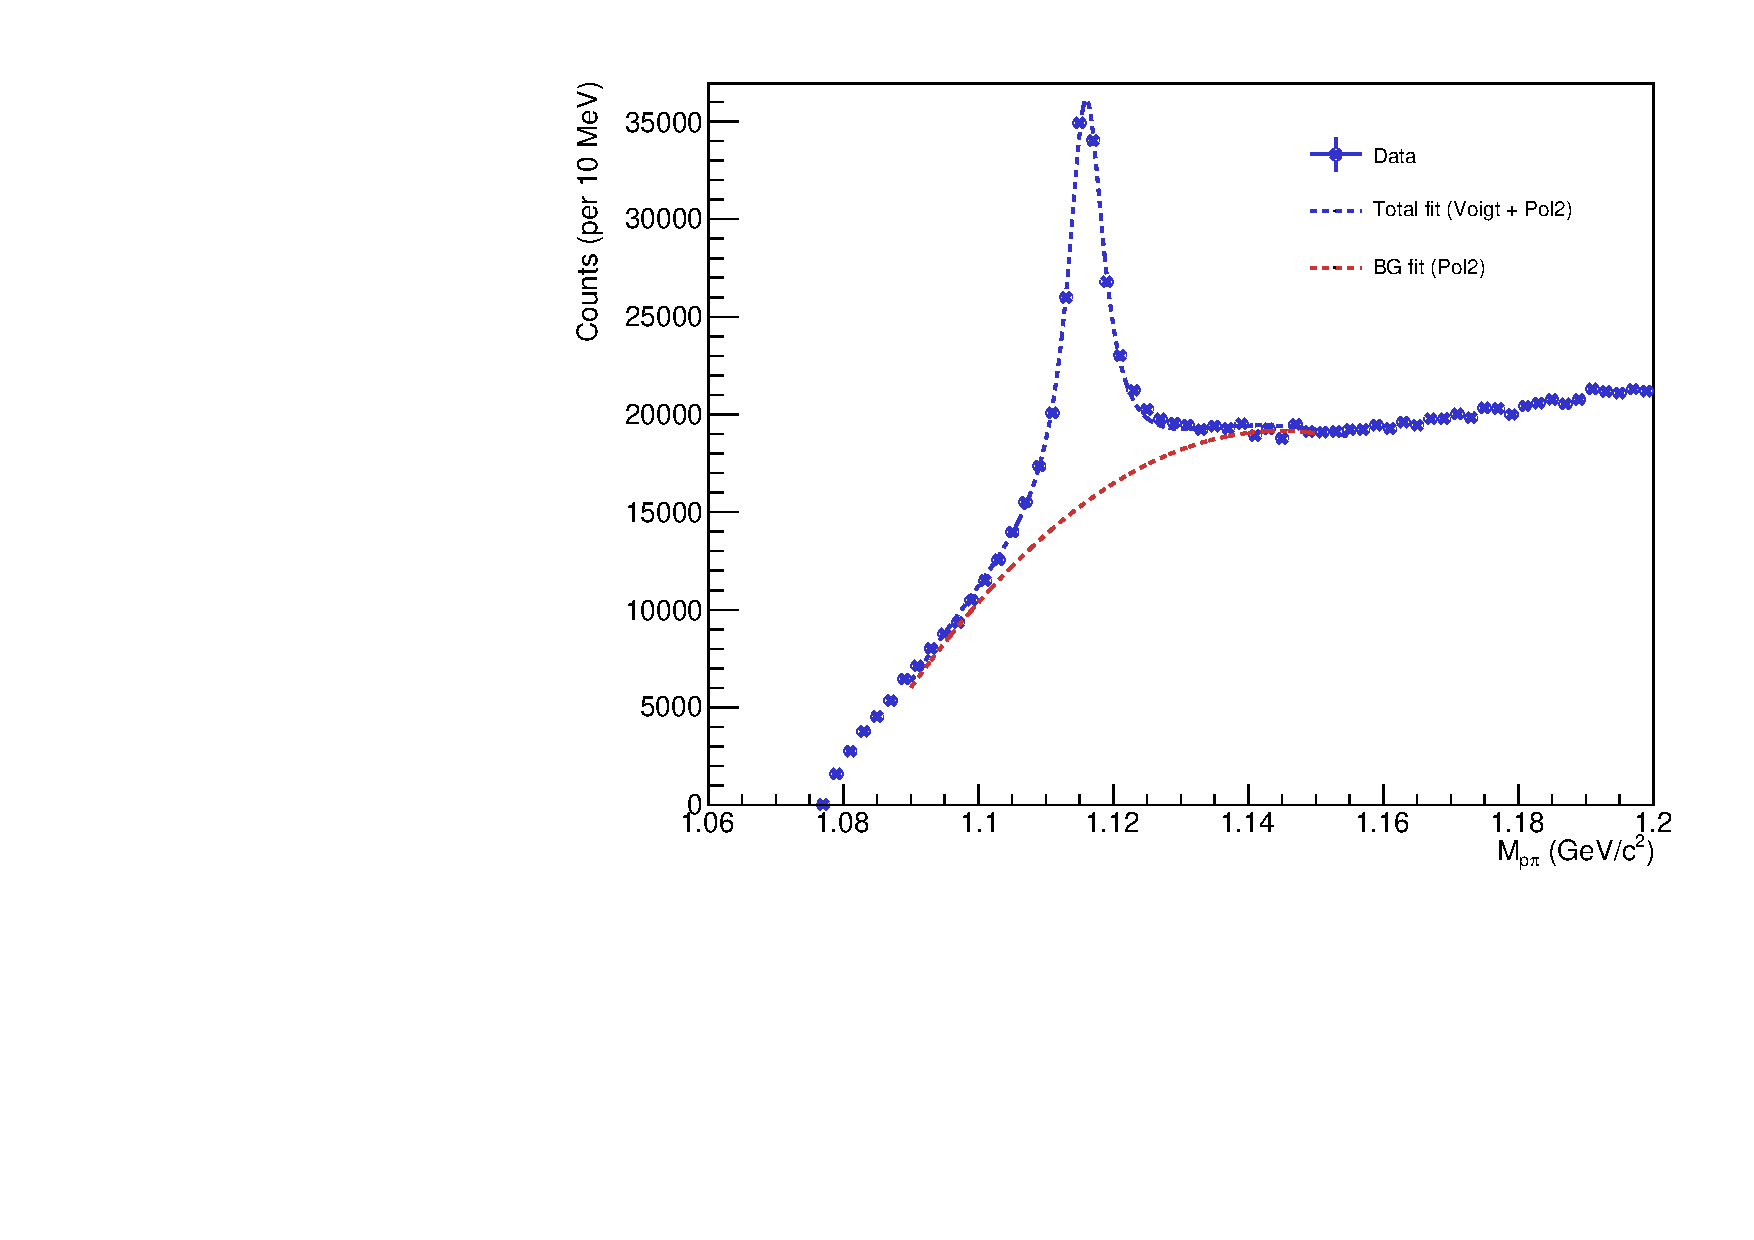
\includegraphics[width=0.48\textwidth]{figures/analysis/lambda_mass_20_50_resonance_fit.pdf}
    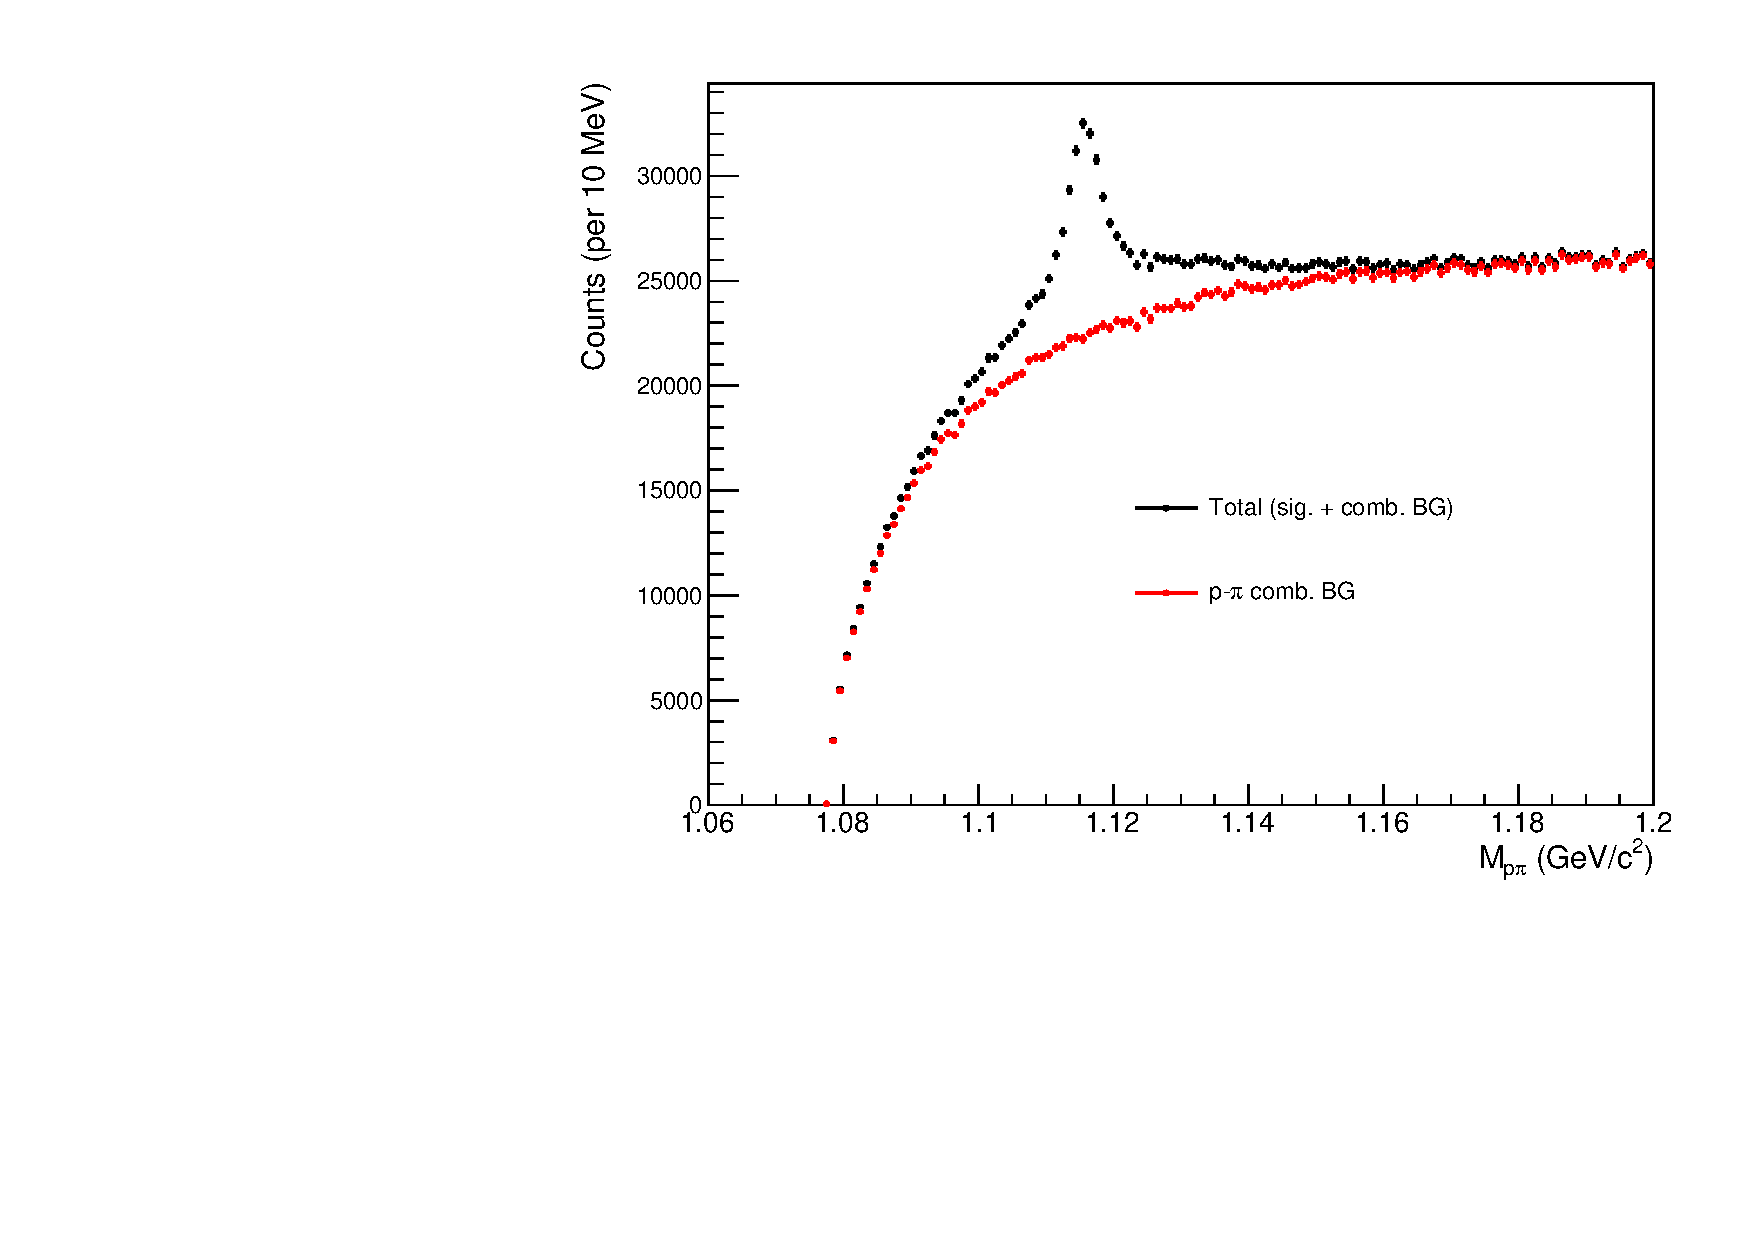
\includegraphics[width=0.48\textwidth]{figures/analysis/lambda_mass_mc_real_bg.pdf}
    \caption{Left: Invariant mass distribution with corresponding Voigt + Polynomial fit in the 20-50\% multiplicity bin (data). Right: The signal and background shapes in MonteCarlo (MC). Note that even though MC appears to have a completely different S/B, the signal shapes should be similar. The fit in data appears to be massively underestimating the $\Lambda$ signal, as the MC sample indicates there is $\Lambda$ signal where the total data fit converges with the BG fit.}
    \label{fig:resonance_fitting_comp}
\end{figure}

This plot shows the main issue with reconstructing \lmb baryons using the resonance technique: the tails of the signal distribution are much wider than the signal distribution obtained using the V$^0$ method. This is due to the fact that the kinematics of the corresponding daughter tracks are calculated assuming they originated from the primary vertex, which is only approximately true in the cases where the \lmb is short-lived. This is different than the \vz method, which calculates the kinematics for the daughter tracks assuming they originated from the secondary vertex. The wider tails of the distribution make it extremely difficult to describe using any common distribution, thus all techniques that rely on fitting the signal shape are not viable. Because of this, only the first two techniques (like-sign and rotated p$\pi$ pairs) will be considered for the rest of this analysis.

To determine which of the two remaining techniques is more effective, the background shape of the $\Lambda$ invariant mass distribution for both techniques in MonteCarlo is compared to the ground-truth background shape. The resulting invariant mass distributions from like-sign and rotated p$\pi$ pairs are shown in Figure \ref{fig:background_approx_MC}, along with a comparison of the extracted signal shapes. 
The LS and rotated p$\pi$ distributions are scaled to match the US distribution in the sideband region, which will be discussed in the next section. The LS p$\pi$ pairs match the background shape of the $\Lambda$ invariant mass distribution more closely than the rotated p$\pi$ pairs, so they are used to estimate the combinatorial background in the $\Lambda$ invariant mass distribution in data.

\begin{figure}[ht]
\centering
    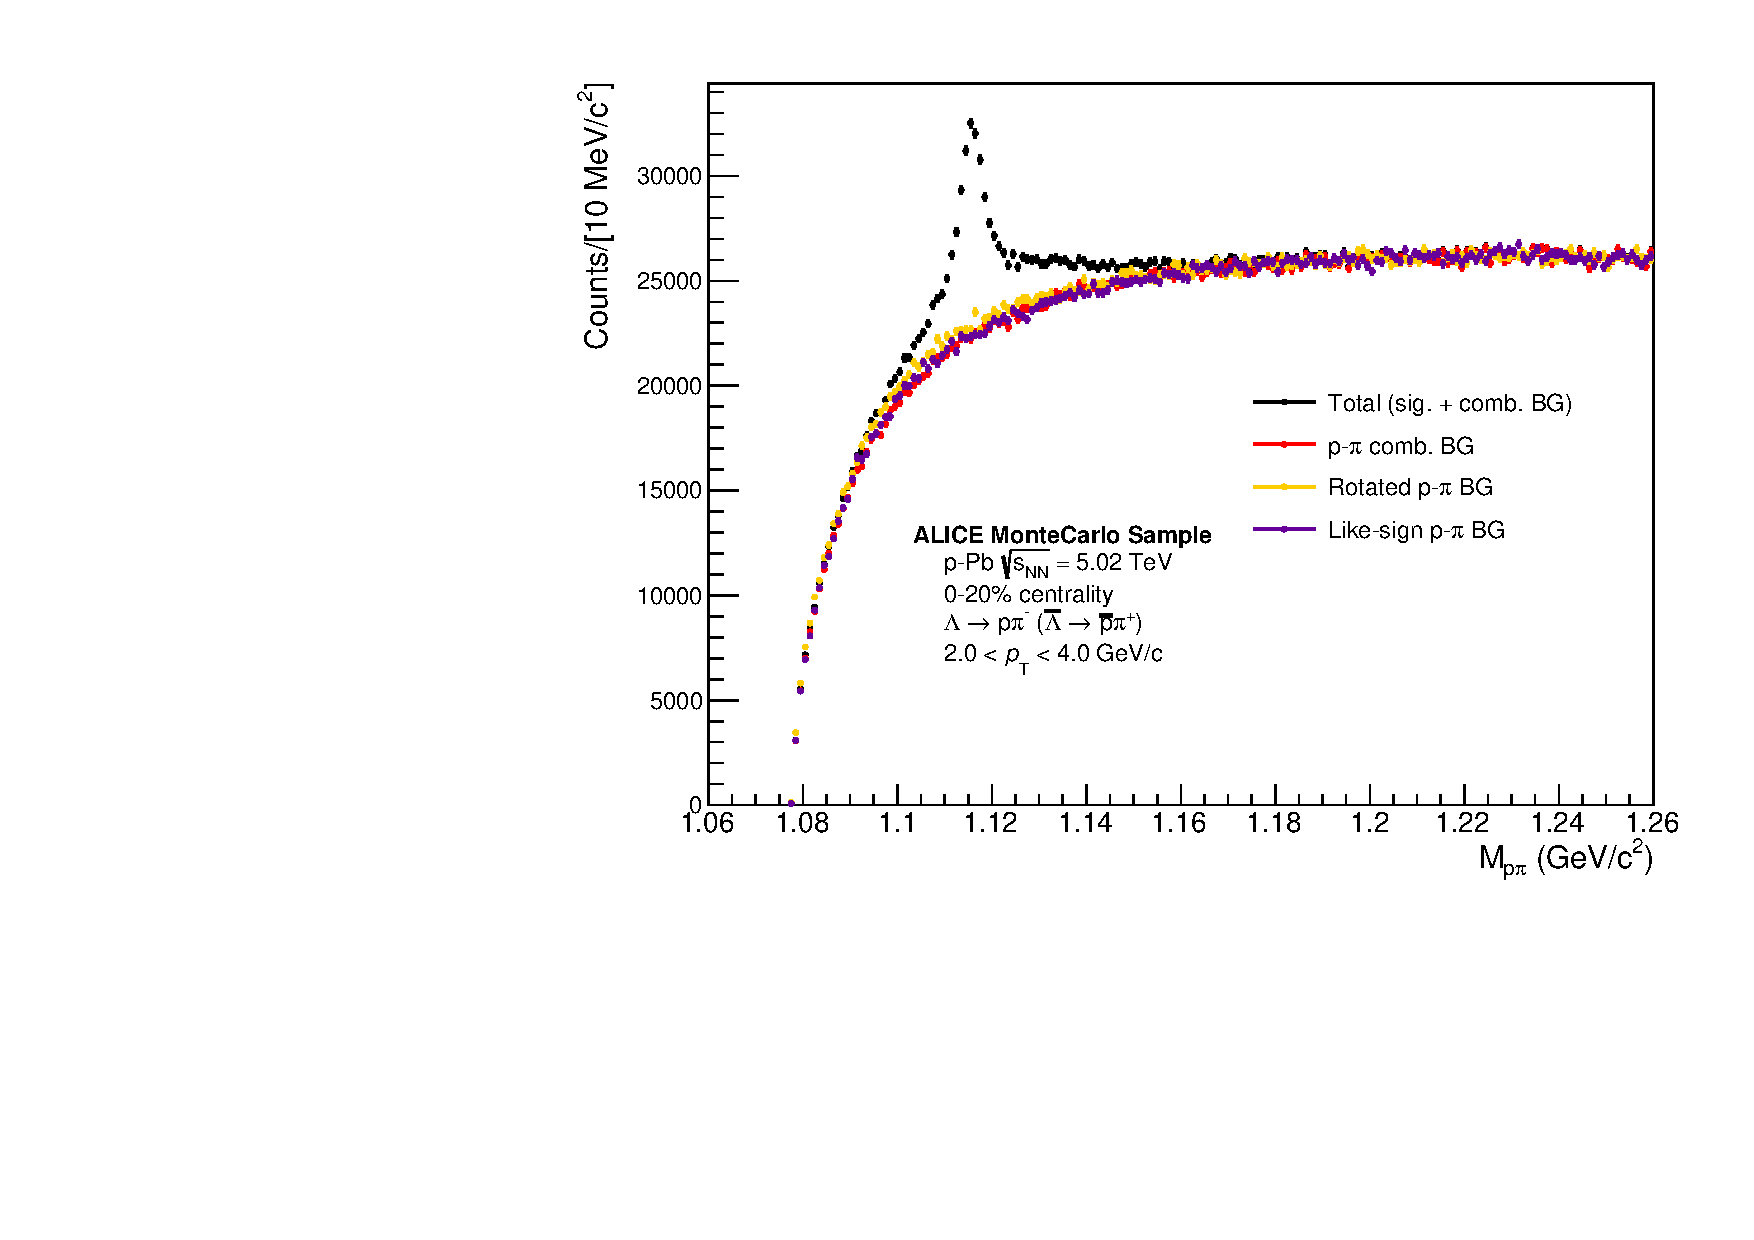
\includegraphics[width=0.48\textwidth]{figures/analysis/background_approx_MC.pdf}
    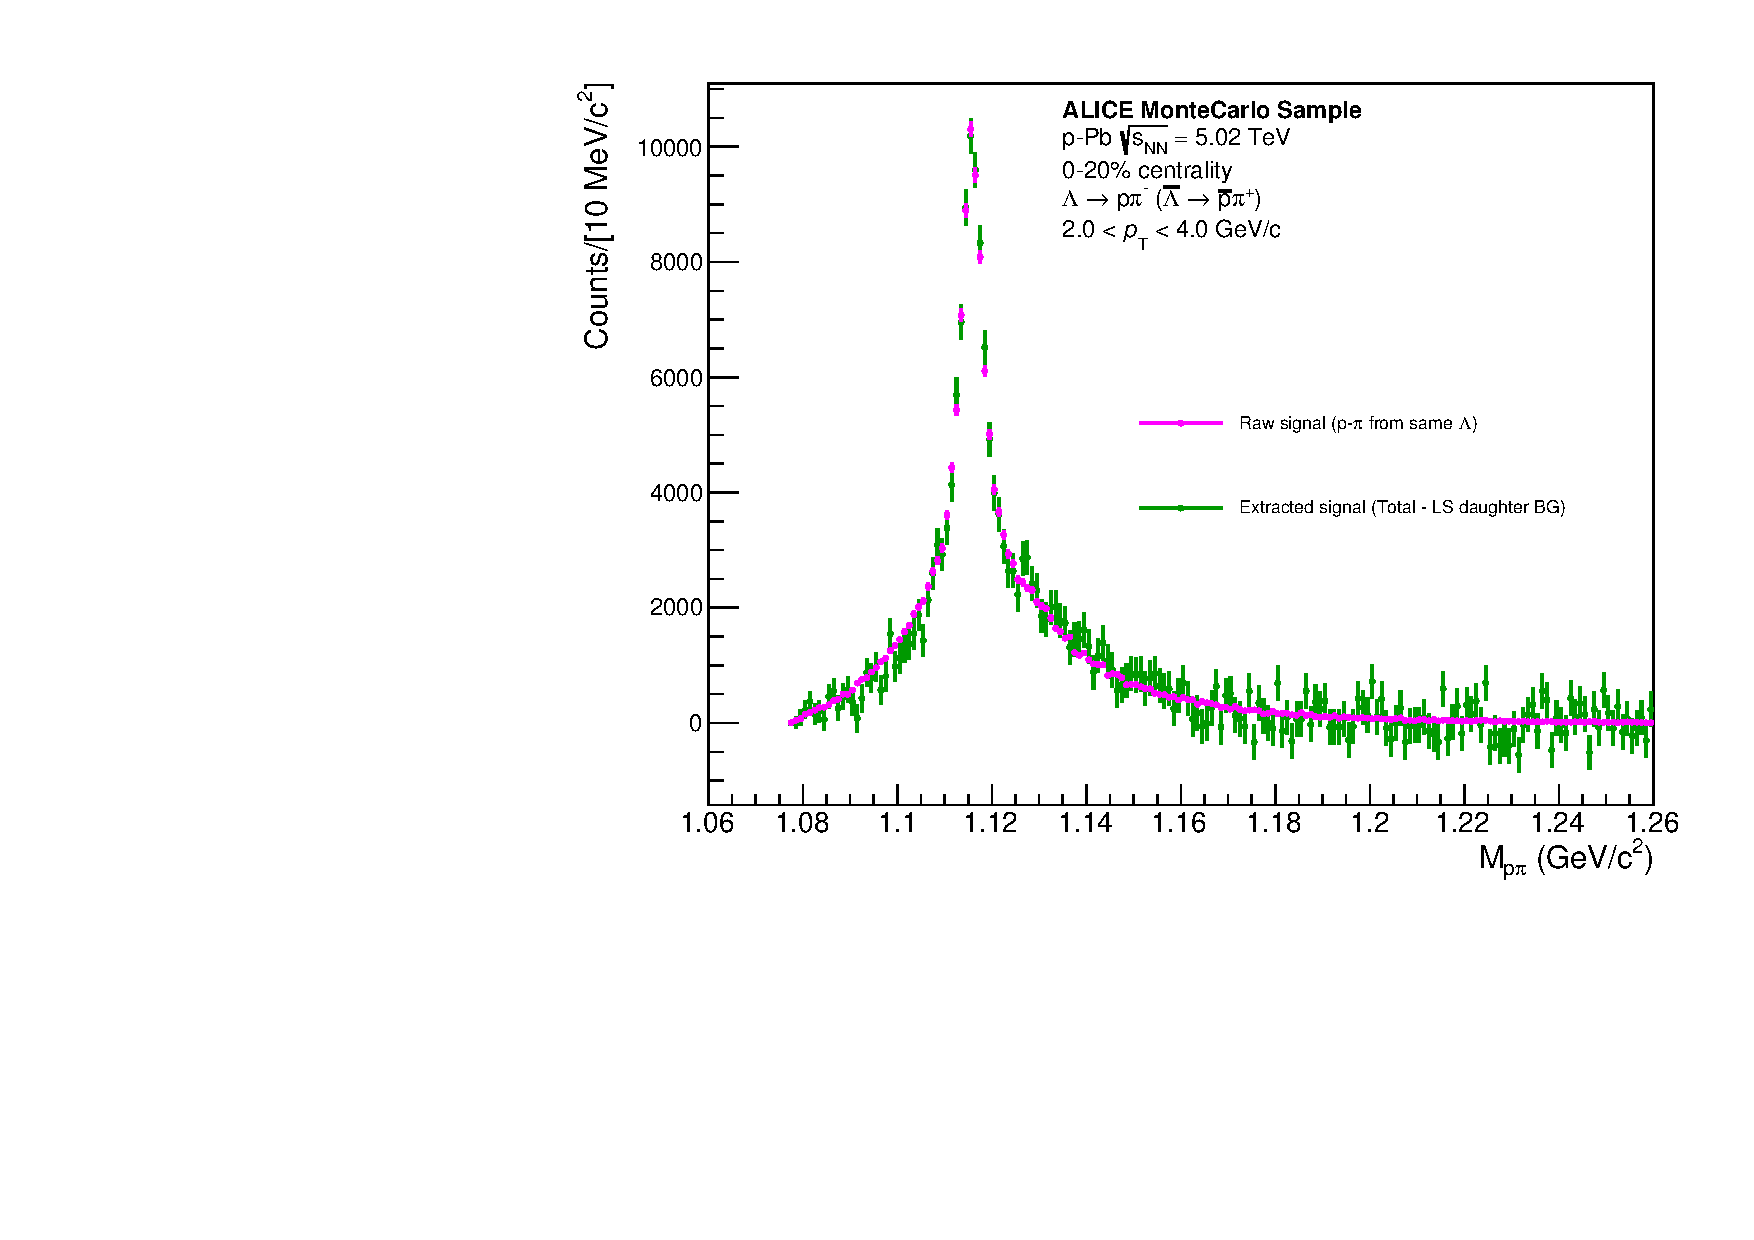
\includegraphics[width=0.48\textwidth]{figures/analysis/background_subtracted_signal_MC.pdf}
    \caption{Left: Invariant mass distribution for reconstructed unlike-sign p$\pi$ pairs (black) in the MonteCarlo sample.  The like-sign p$\pi$ pair mass distribution (purple) and unlike-sign rotated p$\pi$ distributions are scaled to match the unlike-sign distribution outisde of the \lmb signal range. The true combinatorial background (red) matches most closely with the like-sign pairs. Right: The actual $\Lambda$ signal (magenta) compared with the result of subtracting the like-sign from the total unlike-sign p$\pi$ distribution (green). The two distributions show good agreement.}
    \label{fig:background_approx_MC}
\end{figure}
	

\section{Signal and sideband regions}
\label{sec:signal_sideband_res}

As the invariant mass distributions from lambdas reconstructed using the resonance technique are very different from those reconstructed using the \vz technique, so too must the signal and sideband regions be different. The signal region was again chosen to maximize significance across all multiplicity bins, and is defined as the range 1.014 $< M_{\text{p}\pi} < $ 1.026 \GeVmass. Choosing the sideband region is a more complicated procedure, as there is no obvious region in the invariant mass distribution where the signal vanishes. Instead, the sideband region is chosen to minimize the difference between the extracted signal in data and the signal shape in MonteCarlo, which can be seen in Figure \ref{fig:res_invariant_mass_0_20}. The resulting sideband region is 1.160 $< M_{\text{p}\pi} < $ 1.180 \GeVmass.

\begin{figure}[ht]
\centering
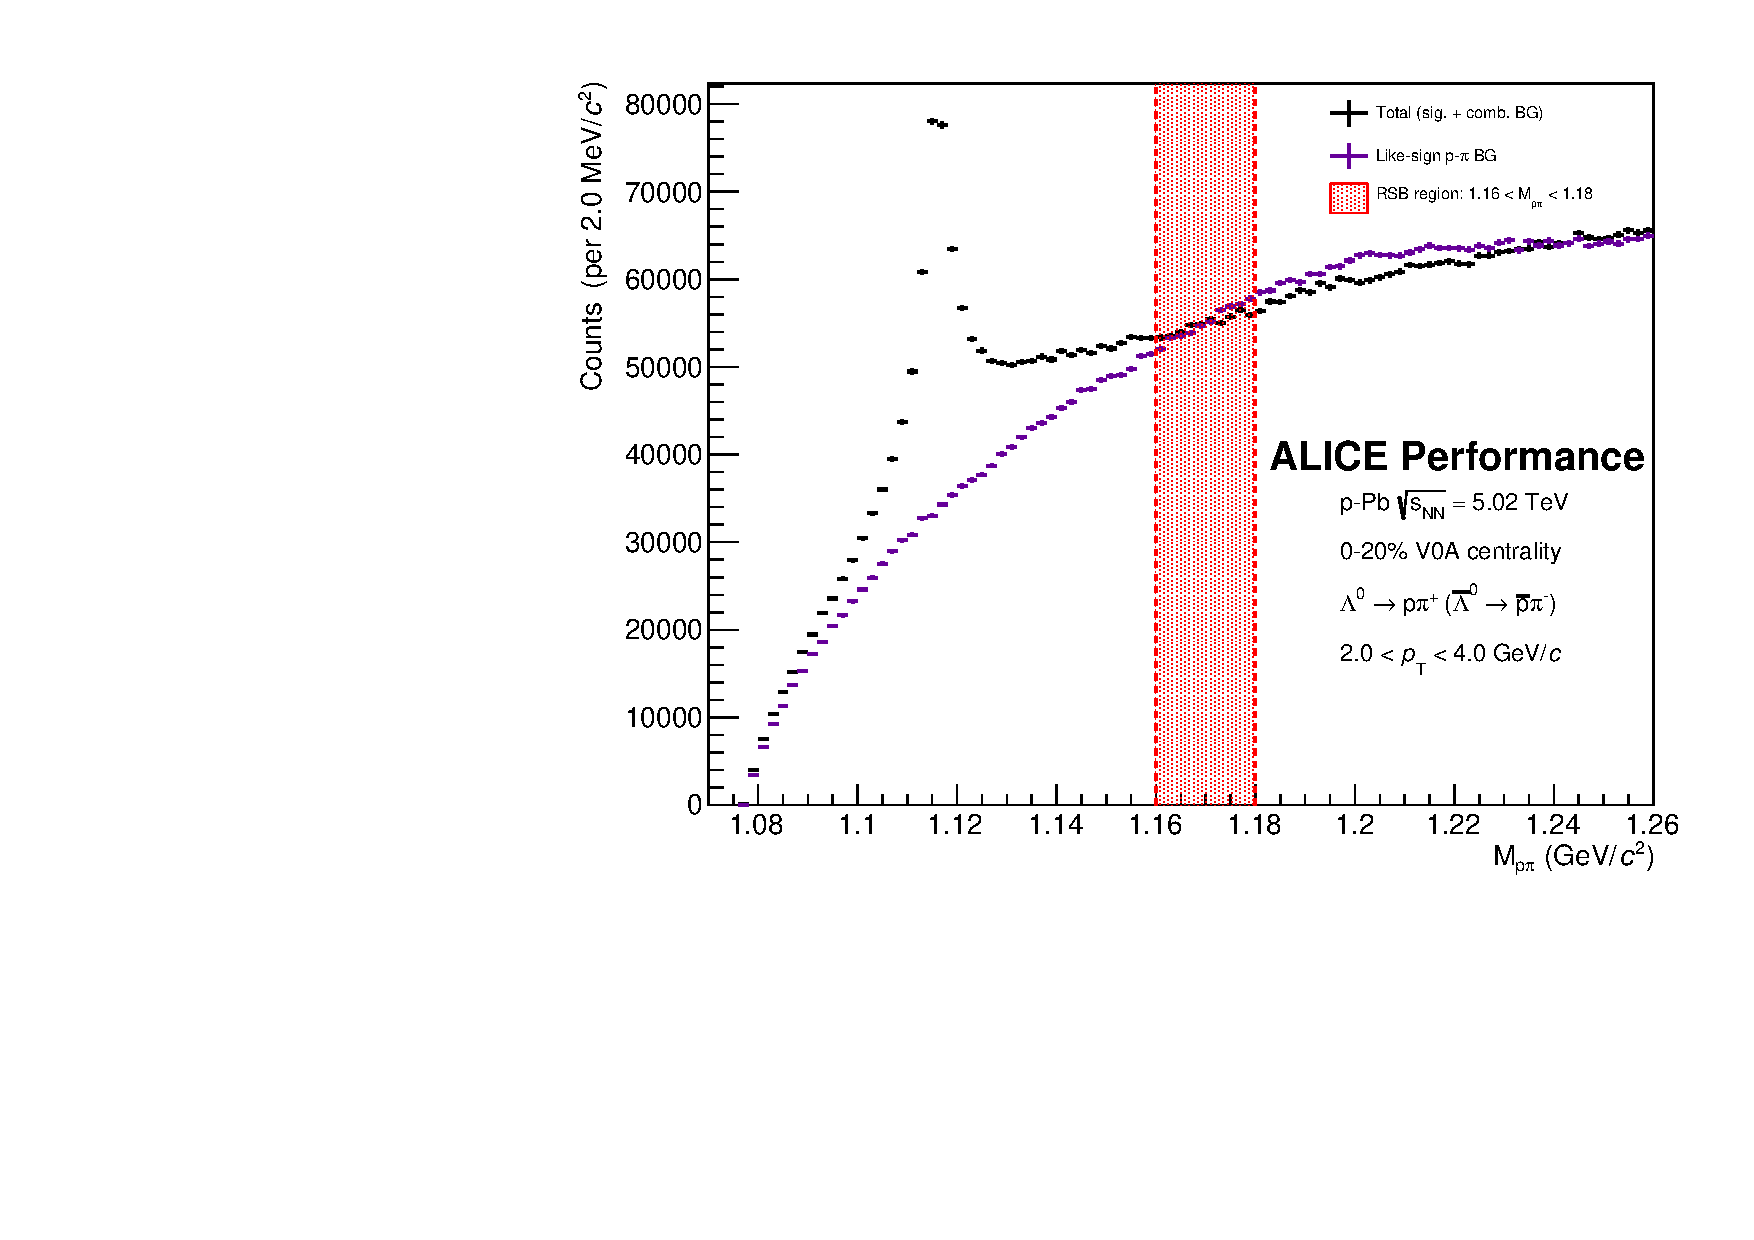
\includegraphics[width=0.48\textwidth]{figures/analysis/lambda_mass_0_20_resonance_with_ls_with_rsb.pdf}
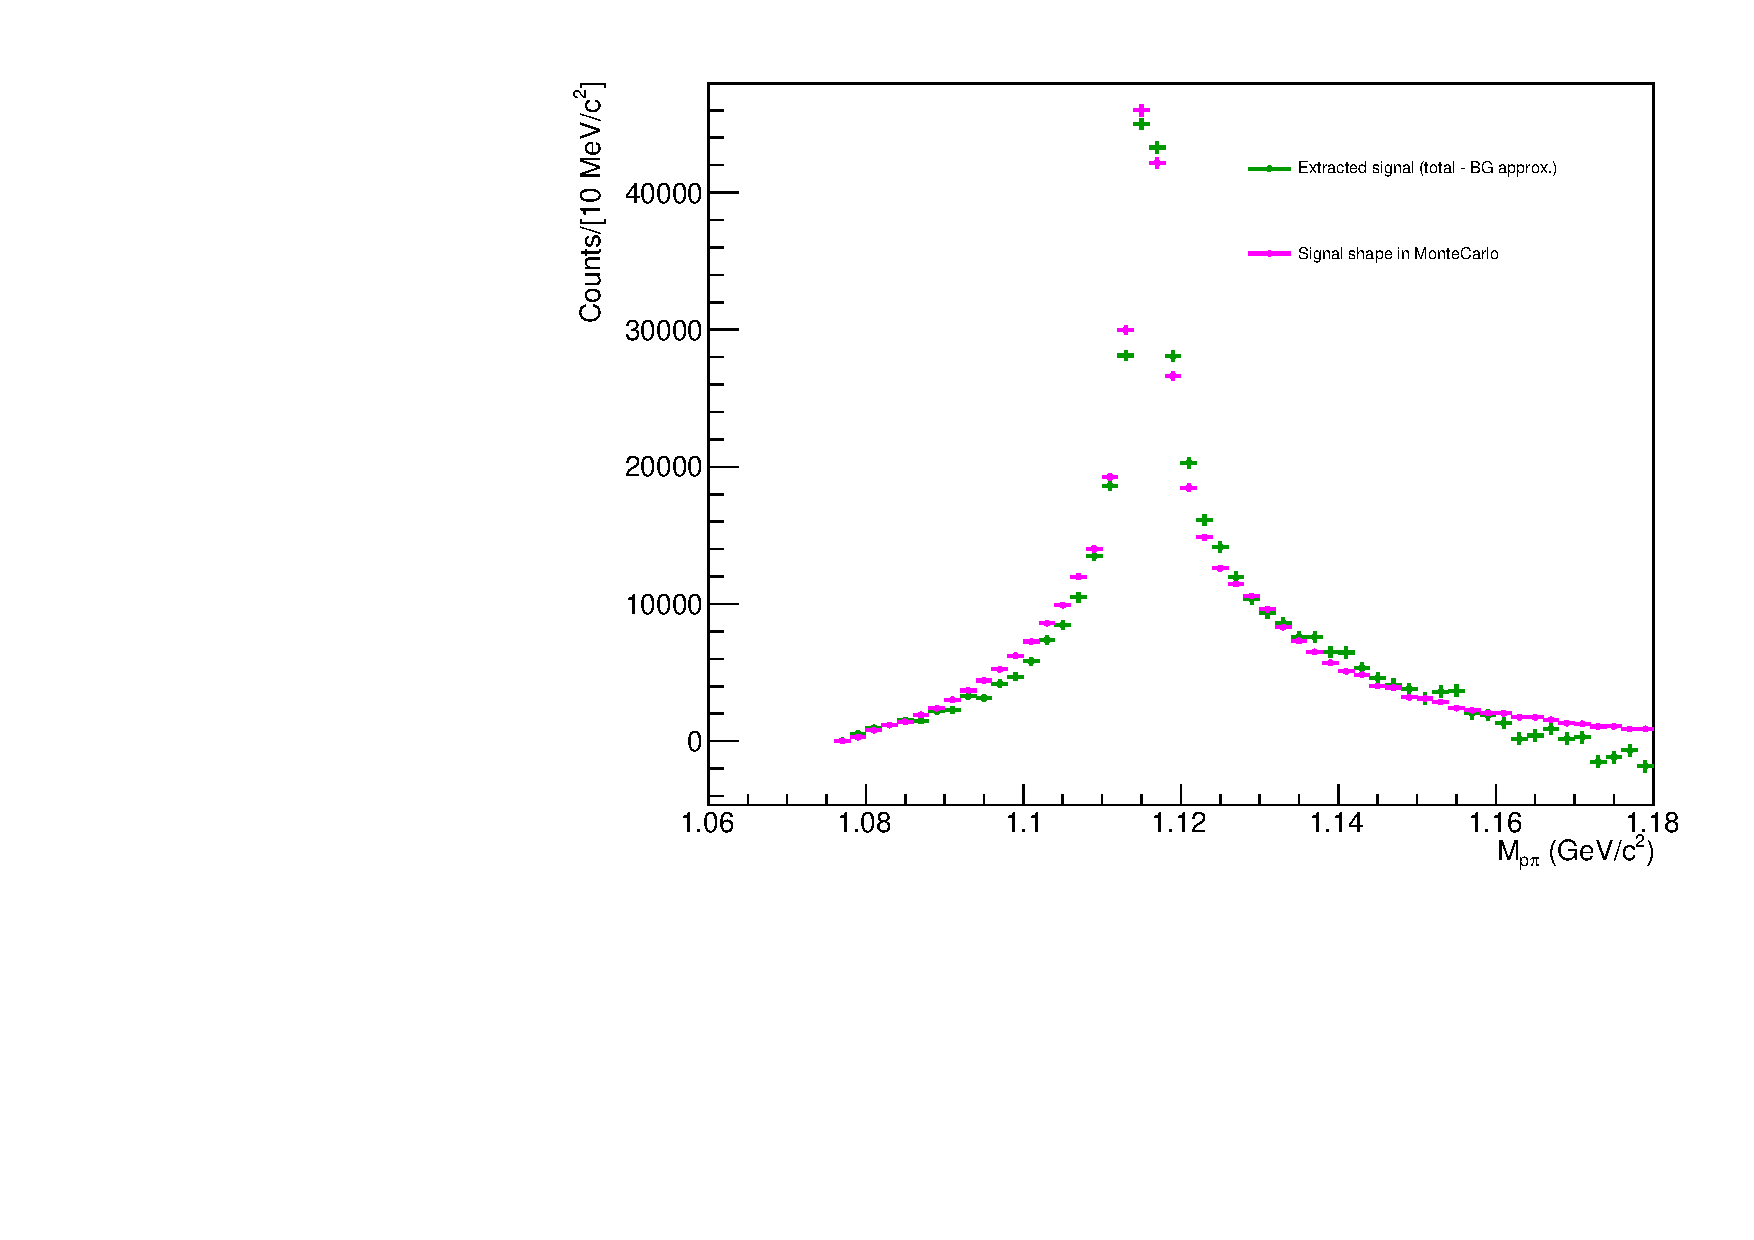
\includegraphics[width=0.48\textwidth]{figures/analysis/lambda_mass_0_20_resonance_signal_comp.pdf}
\caption{Left: Invariant Mass distribution for unlike-sign $p\pi$ pairs (black) along with the like-sign $p\pi$ background (purple) and the sideband region (red) in the 0-20\% multiplicity bin. Right: The extracted signal (green) compared with the resonance-technique reconstructed signal shape in MonteCarlo (magenta). The sideband region was chosen to minimize the differences between these distributions. }
\label{fig:res_invariant_mass_0_20}
\end{figure}

\subsection{Efficiency correction}
Again, the resonance technique-based $\Lambda$ reconstruction efficiency is calculated in a similar manner as the \vz technique, using the formula
%
\begin{equation}
	\epsilon(x_1, x_2, ..., x_n) = \frac{N_{\text{reco.}}(x_1, x_2, ..., x_n)}{N_{\text{gen.}}(x_1, x_2, ..., x_n)},
	\label{eq:efficiency_exp_2}
\end{equation}
%
where $N_{\text{reco.}}$ and $N_{\text{gen.}}$ are the reconstructed and generated particle distributions with kinematic variables $x_1, x_2, ..., x_n$. The main difference from the \vz efficiency computation comes from $N_{\text{reco.}}$, where
each $\Lambda$ candidate is generated using the following procedure:
%
\begin{itemize}
	\item Find all protons and pions within the track list that pass the daughter selection criteria
	\item For each proton in the list, determine if it came from a $\Lambda$ (at generator level)
	\item If the proton came from a $\Lambda$, loop through the pion list until the pion that came from the same $\Lambda$ is found (again, verified at the generator level)
	\item Reconstruct the $\Lambda$ using the daughter tracks found in the previous two steps
	\item Only keep the $\Lambda$ if $|\eta| < 0.8$
\end{itemize}
%
The denominator $N_{\text{gen.}}$ is calculated in the same way as the \vz technique. The resulting efficiency is shown as a function of \pt for each multiplicity bin in Figure \ref{fig:lambda_eff_res}. As expected, the efficiency is higher than the \vz technique, as every \lmb reconstructed using the resonance technique would also be reconstructed using the \vz technique.

\begin{figure}[ht]
    \centering
    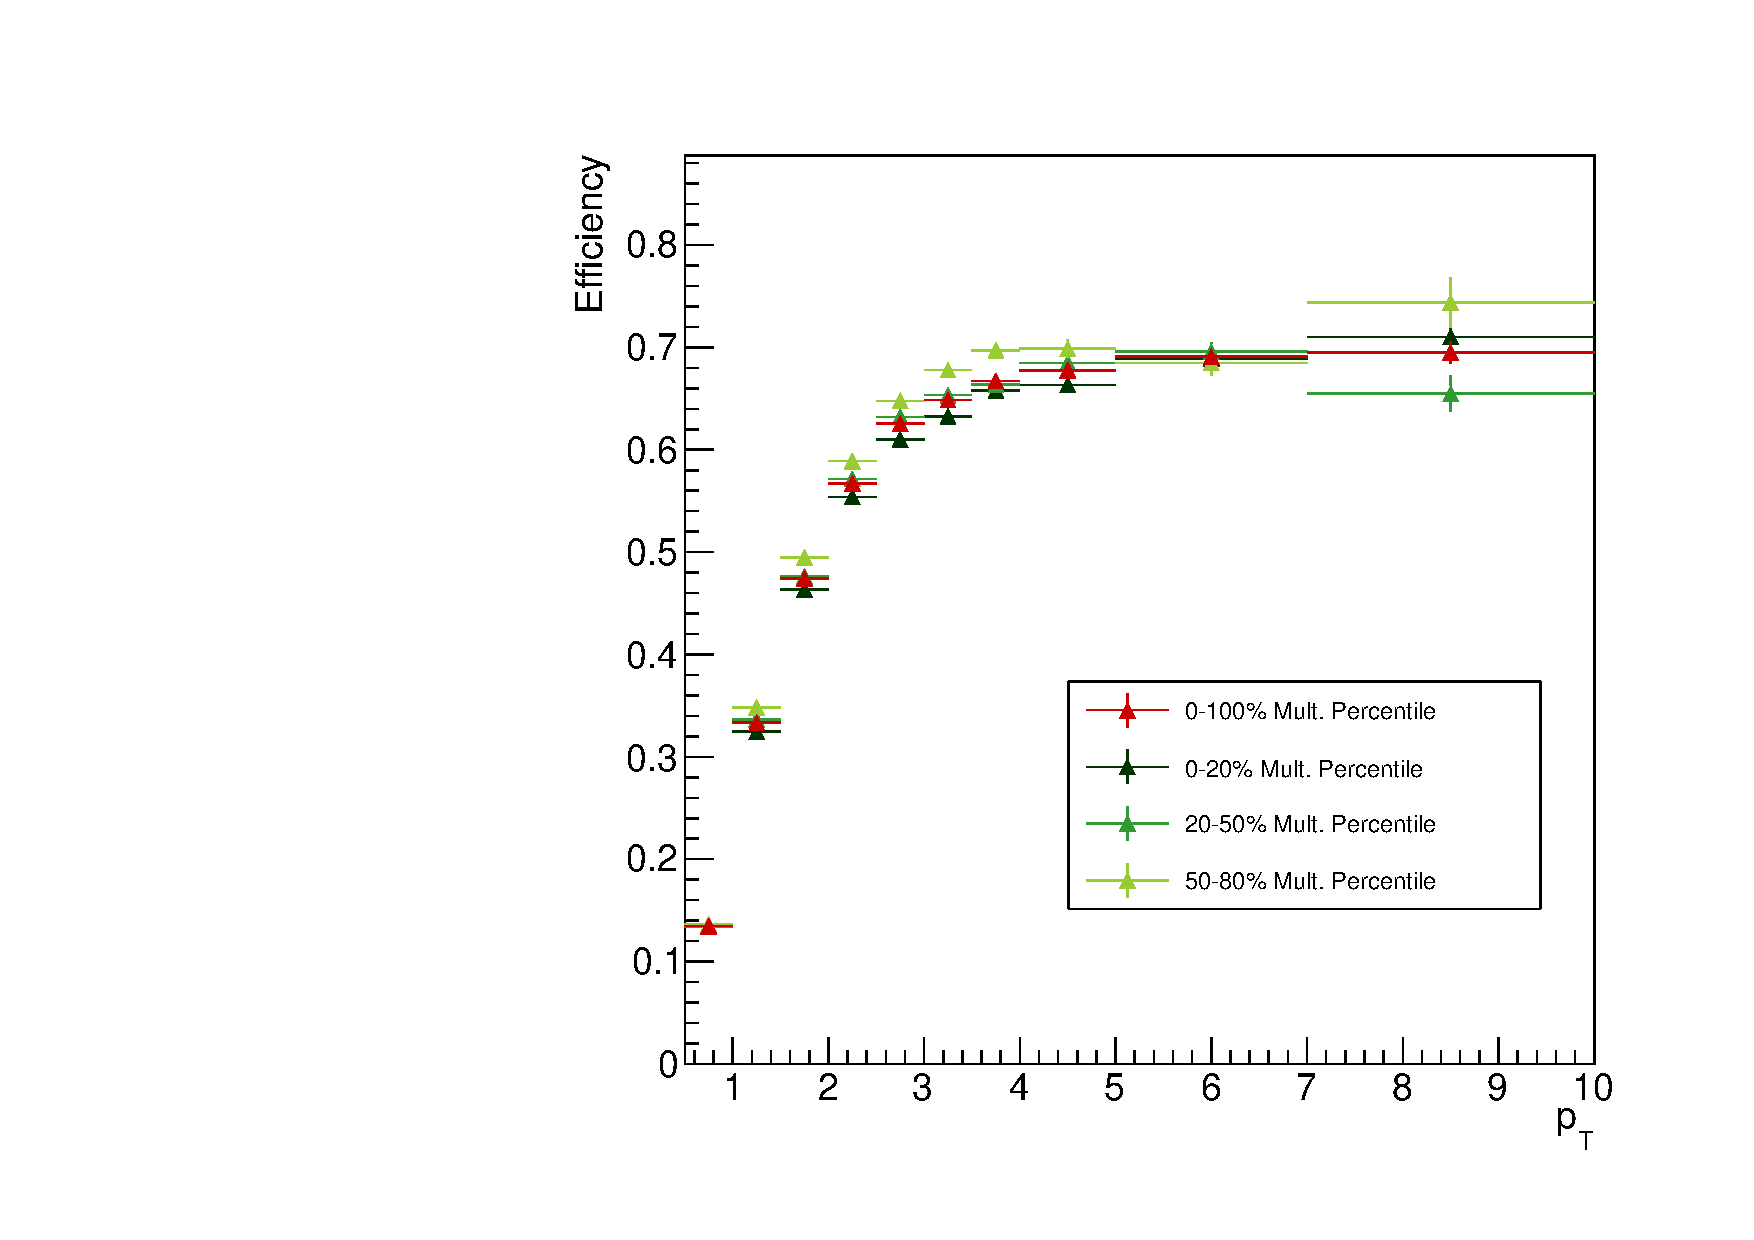
\includegraphics[width=4in]{figures/analysis/res_efficiency.pdf}
    \caption{Efficiency vs. $p_T$ for $\Lambda$ reconstruction using resonance technique for each multiplicity bin, along with an integrated 0-100\% point in red. There does not appear to be any significant dependence on multiplicity. Also worth nothing that the efficiency is higher for this technique when compared to the V0 technique, as expected (all AOD tracks from V0 finder daughters are also in total AOD track list).}
    \label{fig:lambda_eff_res}
\end{figure}

\section{Corrections to the h-\lmb distributions}
\label{sec:removecomb}

All of the efficiency and acceptance corrections are applied to the resonance technique-based h-\lmb distribution in the same way as the \vz technique. The only difference comes from the removal of the combinatorial background, as:
%
\begin{enumerate}
    \item The signal $S$ and background $B$ are calculated in a slightly different manner, and 
    \item The sideband region is vastly different.
\end{enumerate}
%
For the first point, the signal and background are calculated via bin-wise summation of the invariant mass distribution using the LS p$\pi$ pairs as an estimate for the background, scaled to the US distribution in the sideband region.

The second point is mostly inconsequential as the h-p$\pi$ distributions are very similar in a wide range of sideband regions, as shown in Figure \ref{fig:res_sideband_comp}. The nominal sideband region was chosen to be 1.160 $< M_{\text{p}\pi} < $ 1.180 \GeVmass, but any region with a lower bound greater than 1.160 \GeVmass and upper bound less than 1.22 \GeVmass should produce similar results.

\begin{figure}[ht]
    \centering
    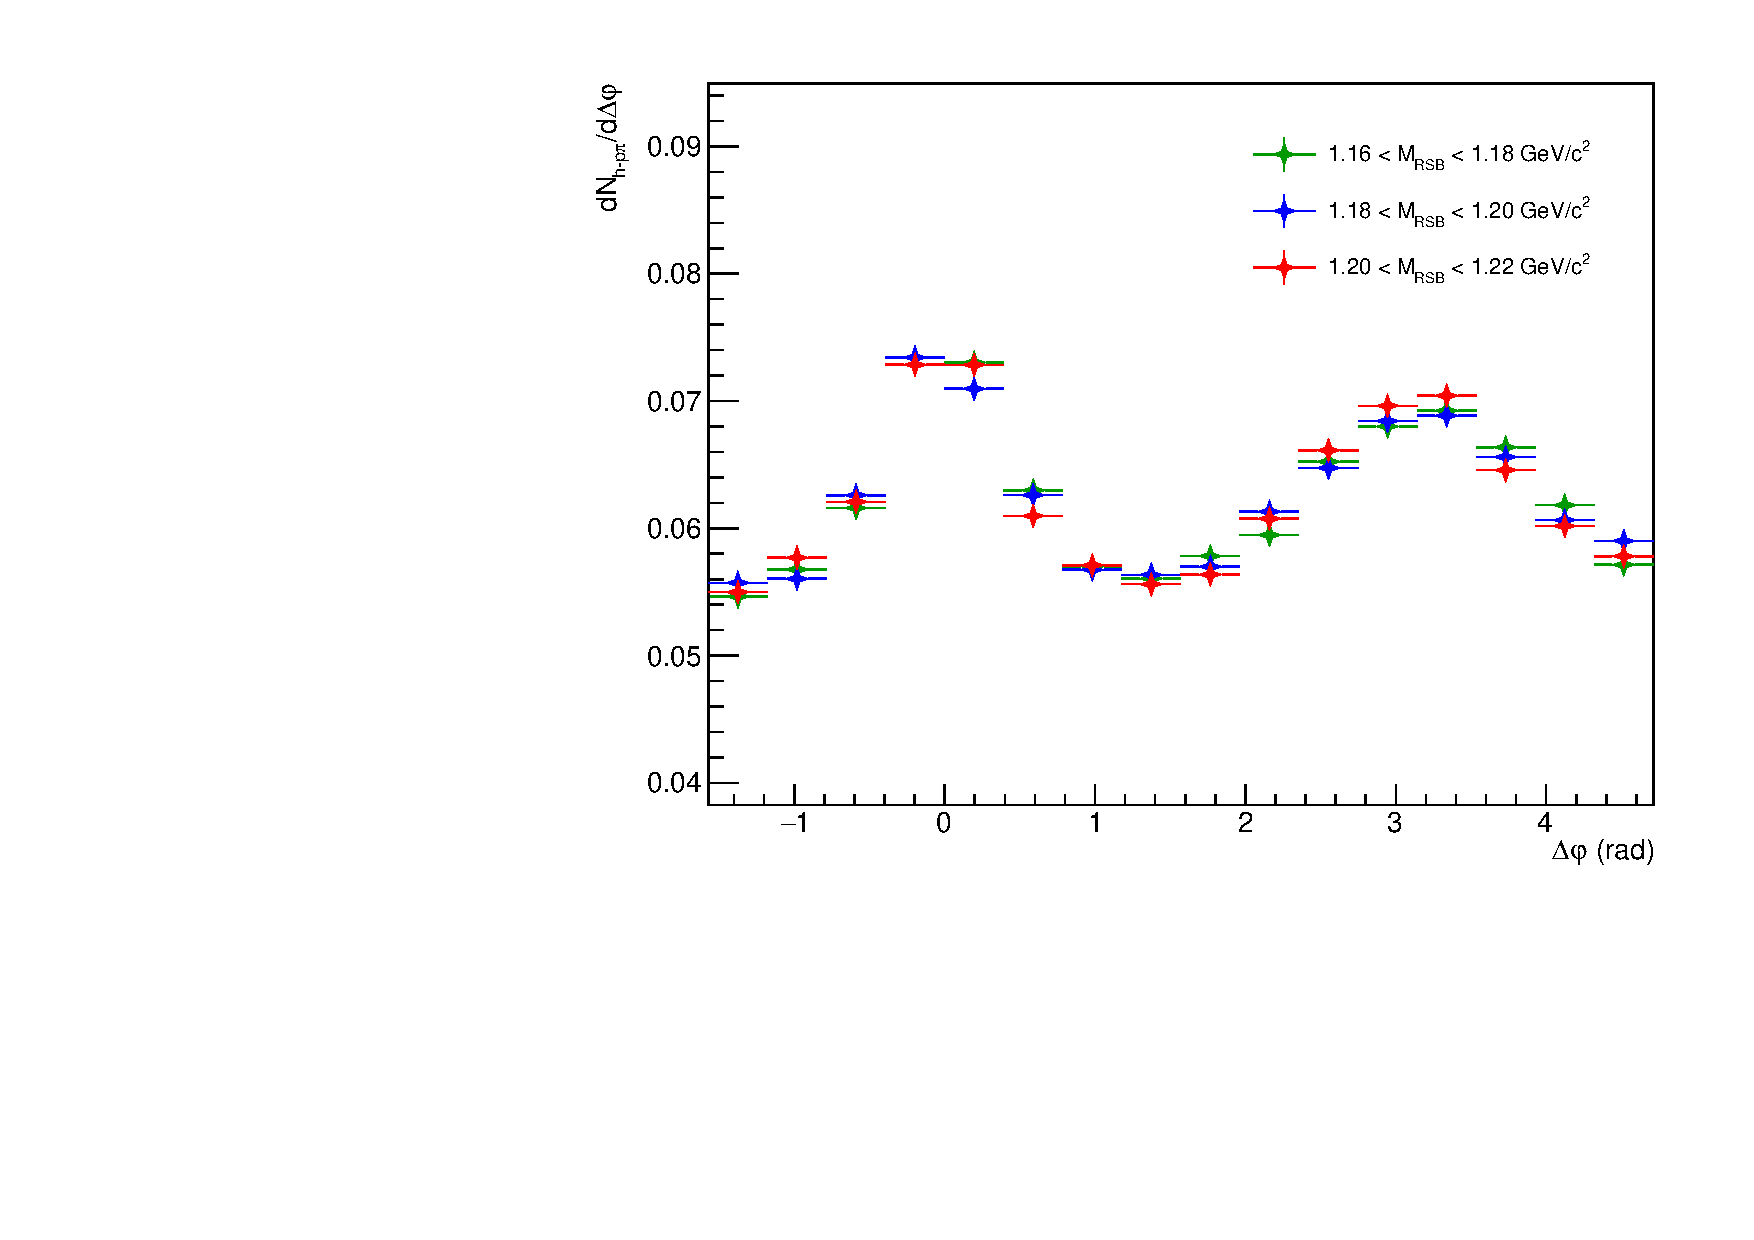
\includegraphics[width=0.5\textwidth]{figures/analysis/h_lambda_dphi_rsbcomp_0_20.pdf}
    \caption{The projected $\Delta\varphi$ distributions for different choices of sideband, taken within the $-1.2 < \Delta\eta < 1.2$ region. The correlation shapes are identical within the statistical errors.}
    \label{fig:res_sideband_comp}
\end{figure}

The signal scaling factor is calculated in the same way as it is in Equation~\ref{eq:signal_scaling}, but with the residual now generated by subtracting the sideband-scaled LS p$\pi$ pairs from the US distribution. The two-track efficiency correction is not applied, as the tools used to calculate the $\epsilon_{\text{pair}}(\Delta\varphi, \Delta\eta)$ template were not developed before the resonance technique-based analysis was completed.

\section{MC closure test}
\label{sec:res_mc_closure}

An MC closure test was also performed for the resonance technique-based analysis, and the results are shown in Figure \ref{fig:res_mc_closure}. The ratio is consistent with unity, but the statistical fluctuations make it difficult to draw any meaningful conclusions. 

\begin{figure}[ht]
    \centering
    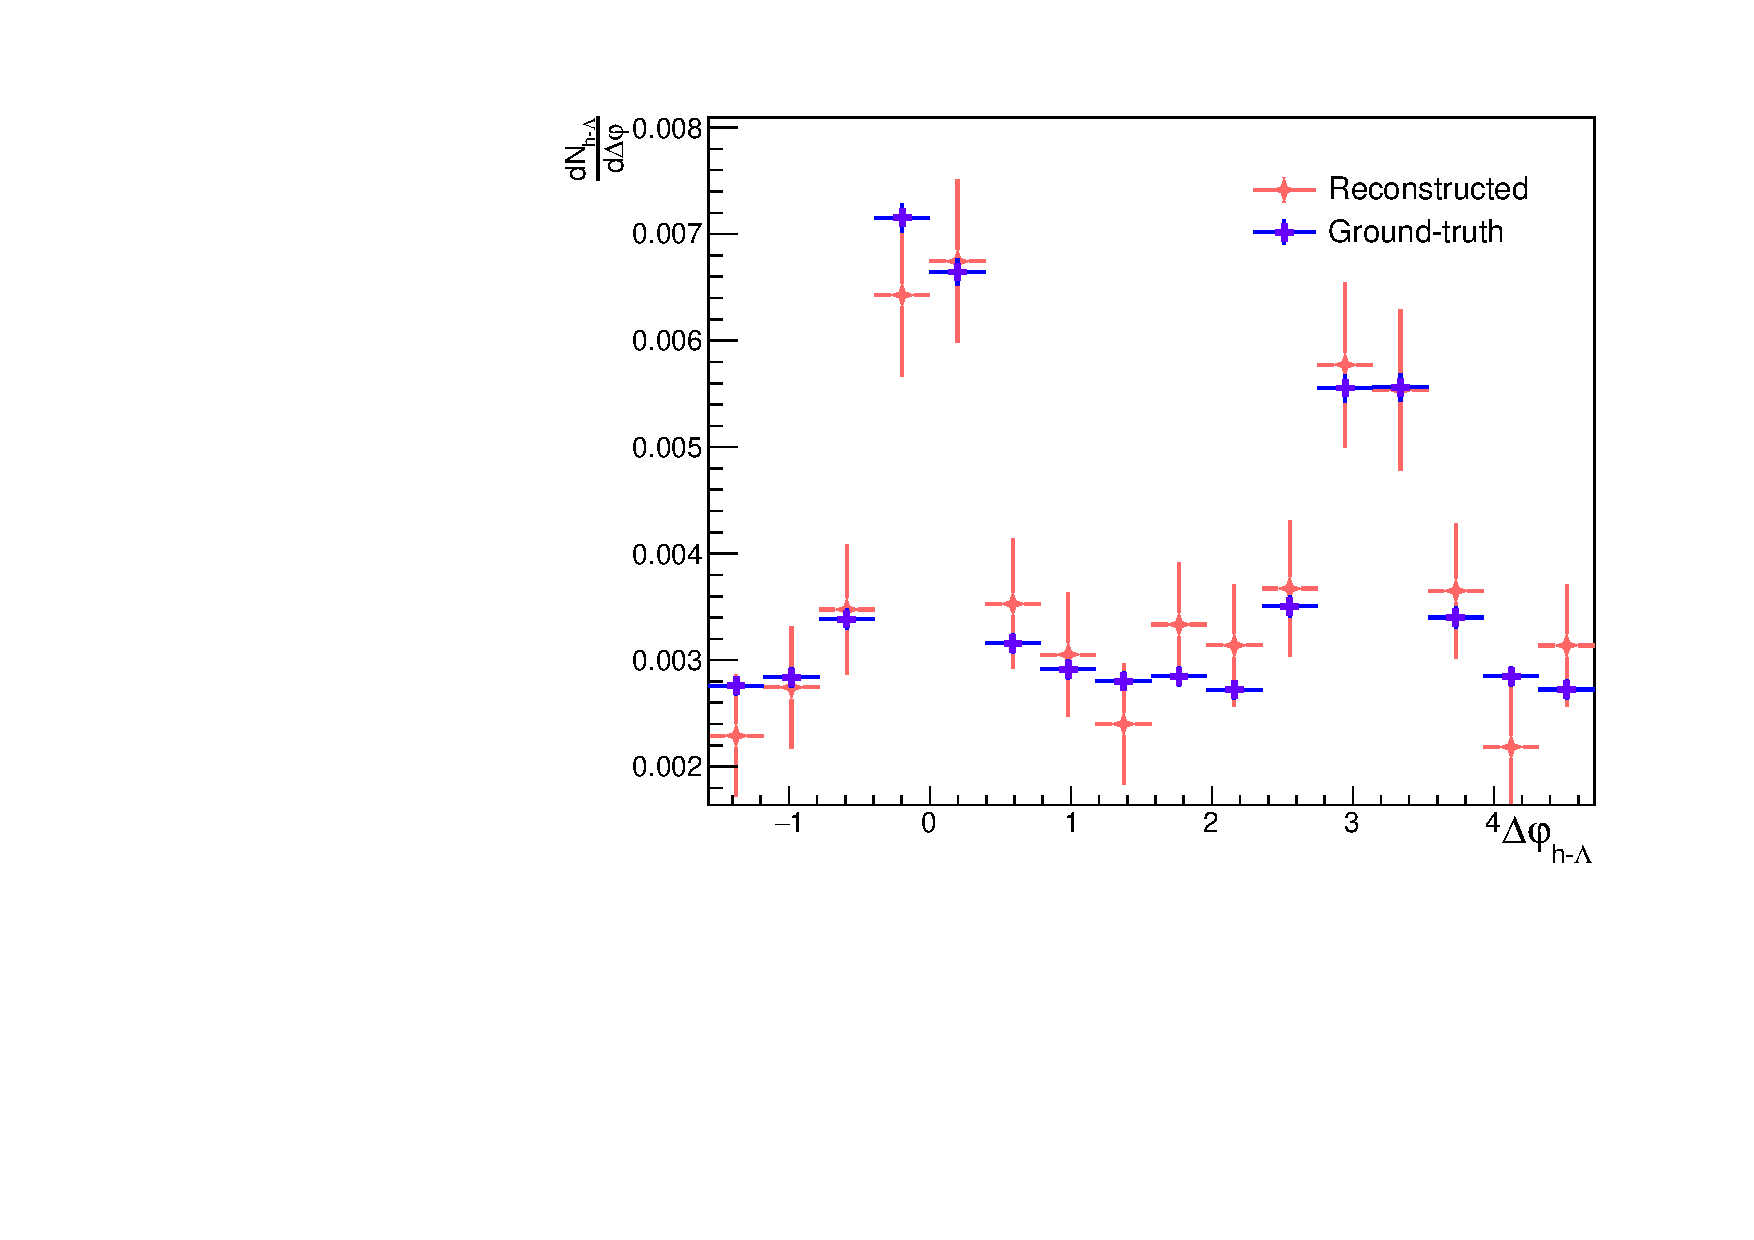
\includegraphics[width=0.48\textwidth]{figures/analysis/h_lambda_mc_closure_res.pdf}
    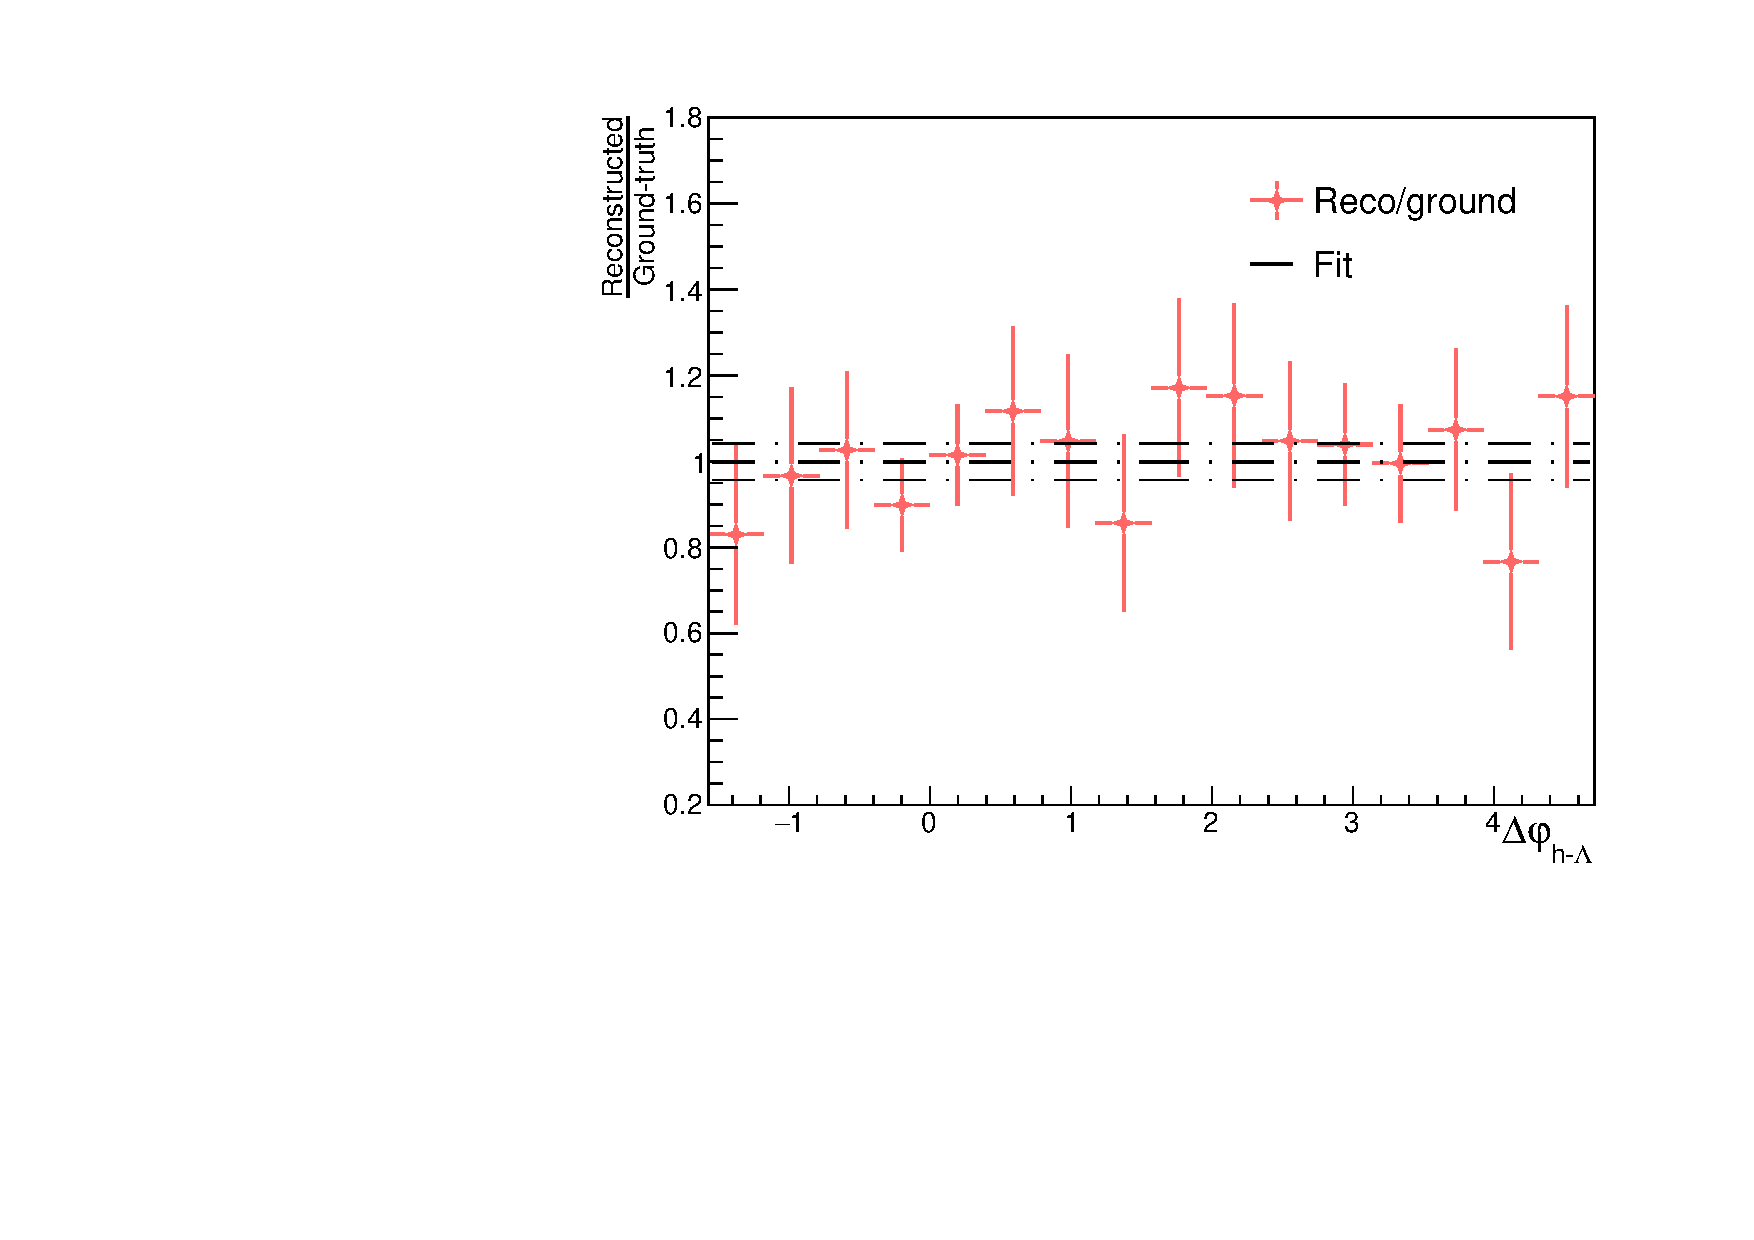
\includegraphics[width=0.48\textwidth]{figures/analysis/h_lambda_mc_closure_ratio_res.pdf}
    \caption{The reconstructed (red) and ground-truth (blue) h-$\Lambda_{\text{res}}$ $\Delta\varphi$ distributions along with a (reconstructed)/(ground-truth) ratio and straight-line fit. The fit is technically consistent with unity, but the statistical fluctuations are quite large.}
    \label{fig:res_mc_closure}
\end{figure}

As the reconstructed distribution has not been corrected for the two-track merging effect, it is surprising that the ratio does not exhibit a significant deviation from unity at small $\Delta\varphi$. This is likely due to two factors:
%
\begin{enumerate}
\item The resonance technique has a much lower S/B, and therefore the sideband subtraction introduces a large amount of statistical fluctuations making such deviations difficult to observe, and
\item The reconstructed daughter tracks have a larger fraction of higher quality tracks when compared to the  \vz technique, and those tracks are less likely to be merged over by the trigger during reconstruction.
\end{enumerate}
%
To elaborate on the second point, while the resonance and \vz techniques use the same loose quality cuts, the daughter tracks coming from the \vz technique must have a resolvable secondary vertex, which biases the corresponding \lmb sample to those with a higher decay length. As discussed in~\ref{sec:pair_eff_corr}, the two-track merging effect is more pronounced at larger decay lengths, thus the h-\lmb distributions using the \vz reconstruction technique will have a larger fraction of merged tracks when compared to the resonance technique-based distributions.

To further investigate this surprising closure of the resonance technique-based h-$\Lambda$ $\Delta\varphi$ distributions, the same closure test is performed, but for the reconstructed h-$\Lambda$ distribution, the $\Lambda$ candidate is required to have have a corresponding particle at the generator-level, making the combinatorial background exactly zero and removing the need for sideband subtraction. The results of this test are shown in Figure \ref{fig:h_lambda_mc_closure_res_no_sideband}. The ratio is no longer consistent with unity at small $\Delta\varphi$, as expected\footnote{It is strange to \textit{want} non-closure, but it would be even stranger if the track merging effect were somehow not present in the resonance technique-based analysis.}

\begin{figure}[ht]
    \centering
    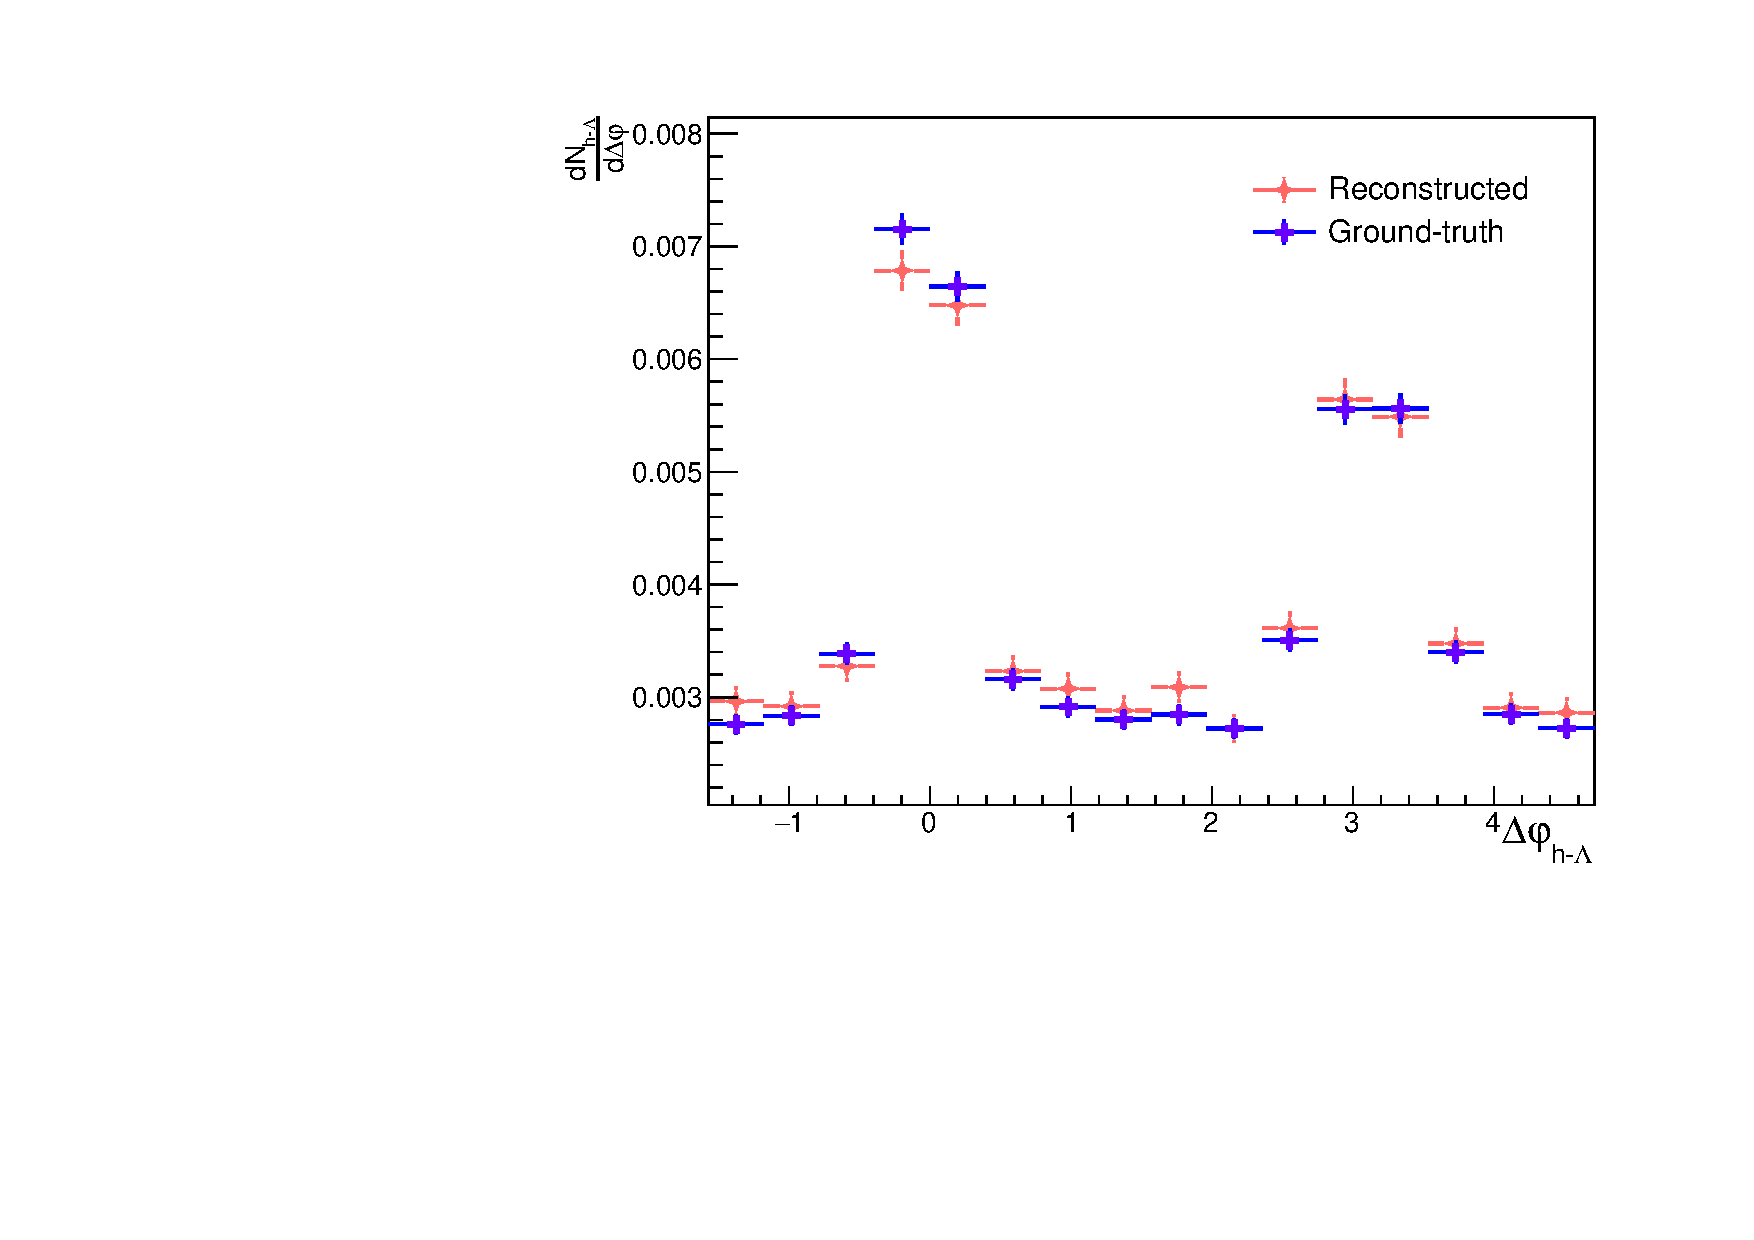
\includegraphics[width=0.48\textwidth]{figures/analysis/h_lambda_mc_closure_res_no_sideband.pdf}
    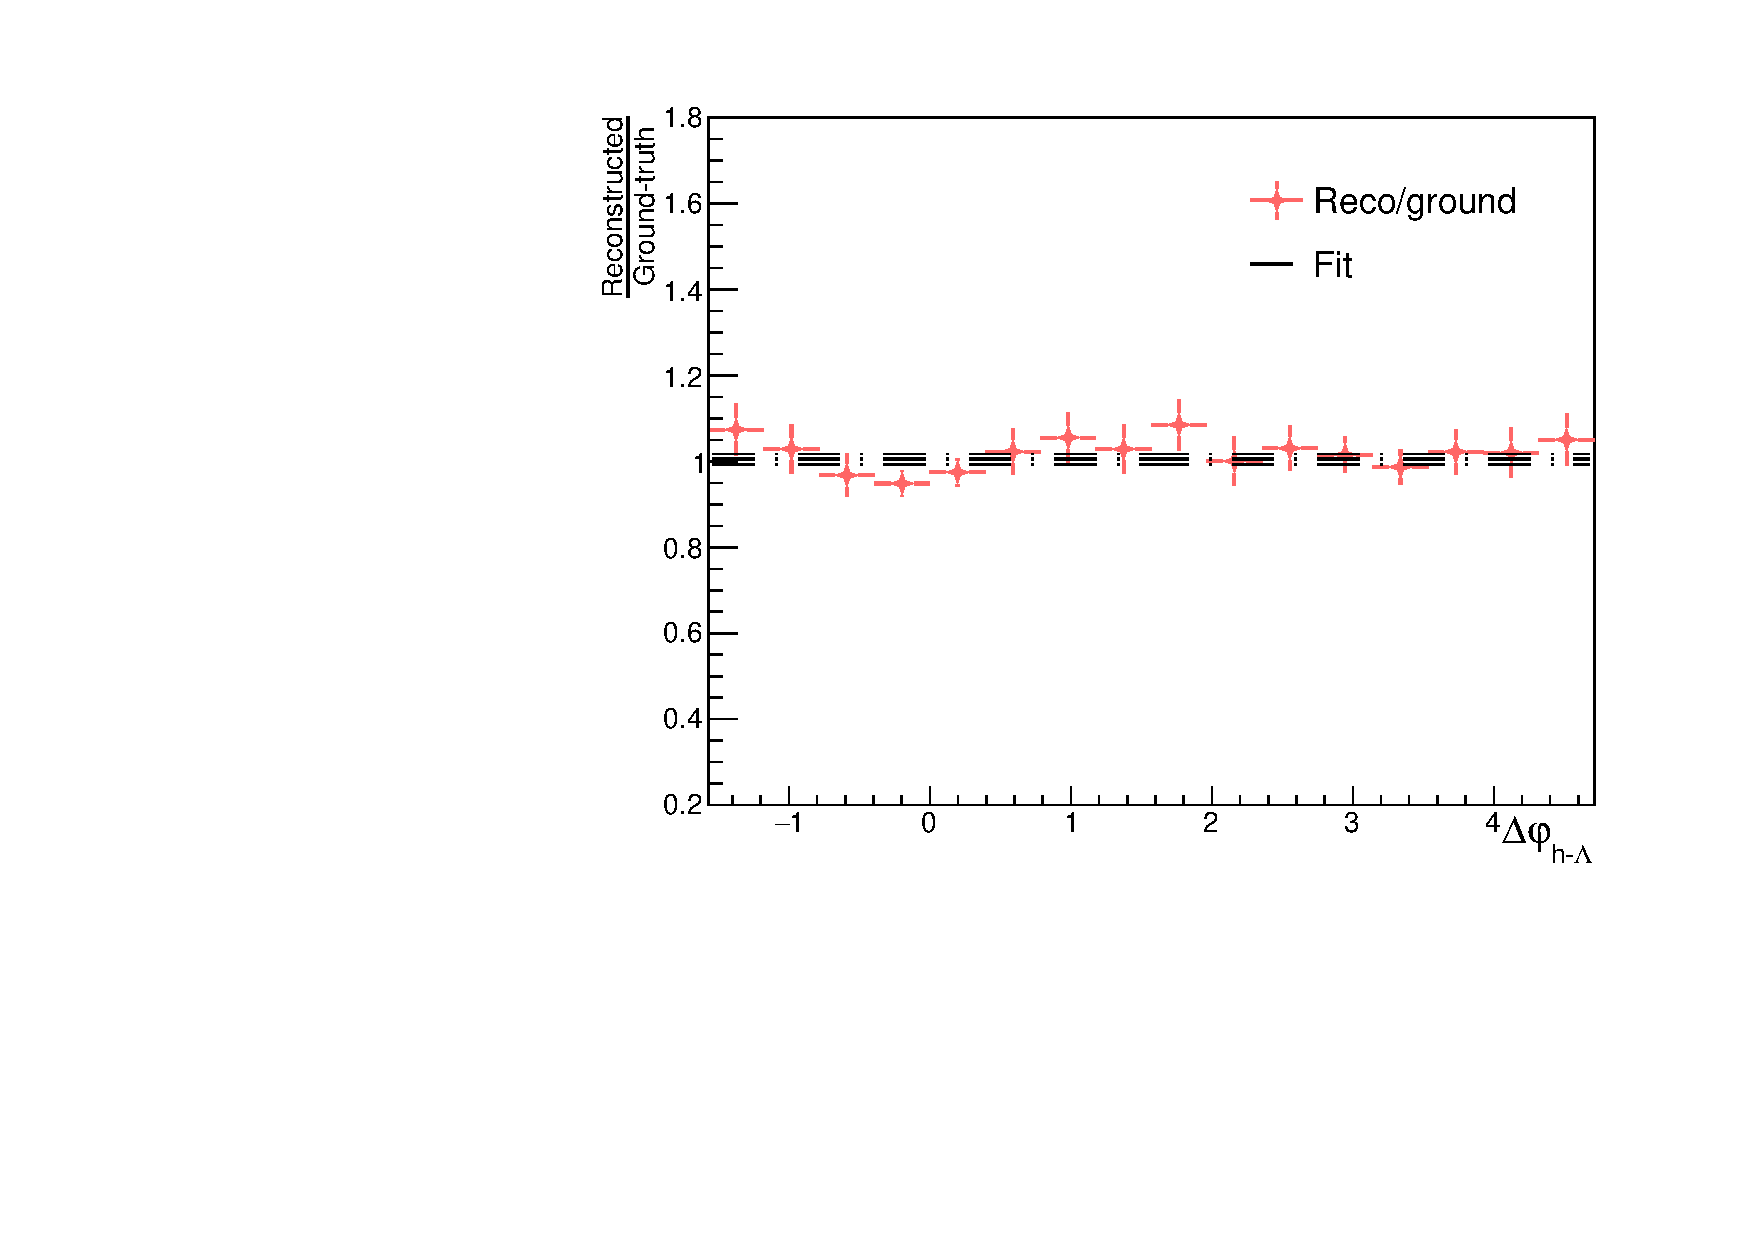
\includegraphics[width=0.48\textwidth]{figures/analysis/h_lambda_mc_closure_ratio_res_no_sideband.pdf}
    \caption{The reconstructed (red) and ground-truth (blue) h-$\Lambda_{\text{res}}$ $\Delta\varphi$ distributions along with a (reconstructed)/(ground-truth) ratio and straight-line fit, but instead requiring the reconstructed $\Lambda$ to have a corresponding particle at the generator level to make sideband subtraction unnecessary.  The result is no longer consistent with unity at small $\Delta\varphi$ due to the track merging effect, but the non-closure is much smaller than the V0 technique.}
    \label{fig:h_lambda_mc_closure_res_no_sideband}
\end{figure}


\section{Some additional results}


A comparison of the final per-trigger h-$\Lambda$ $\Delta\varphi$ correlation structure from the resonance and \vz-based techniques was shown in Chapter~\ref{chapter_systematics}, but it can be seen again in Figure \ref{fig:resonance_v0_dphi_comp_2}. As mentioned previously, the correlation shapes are nearly identical, with the resonance technique having slightly larger uncertainties due to the combinatorial background subtraction. 

\begin{figure}[h]
    \centering
    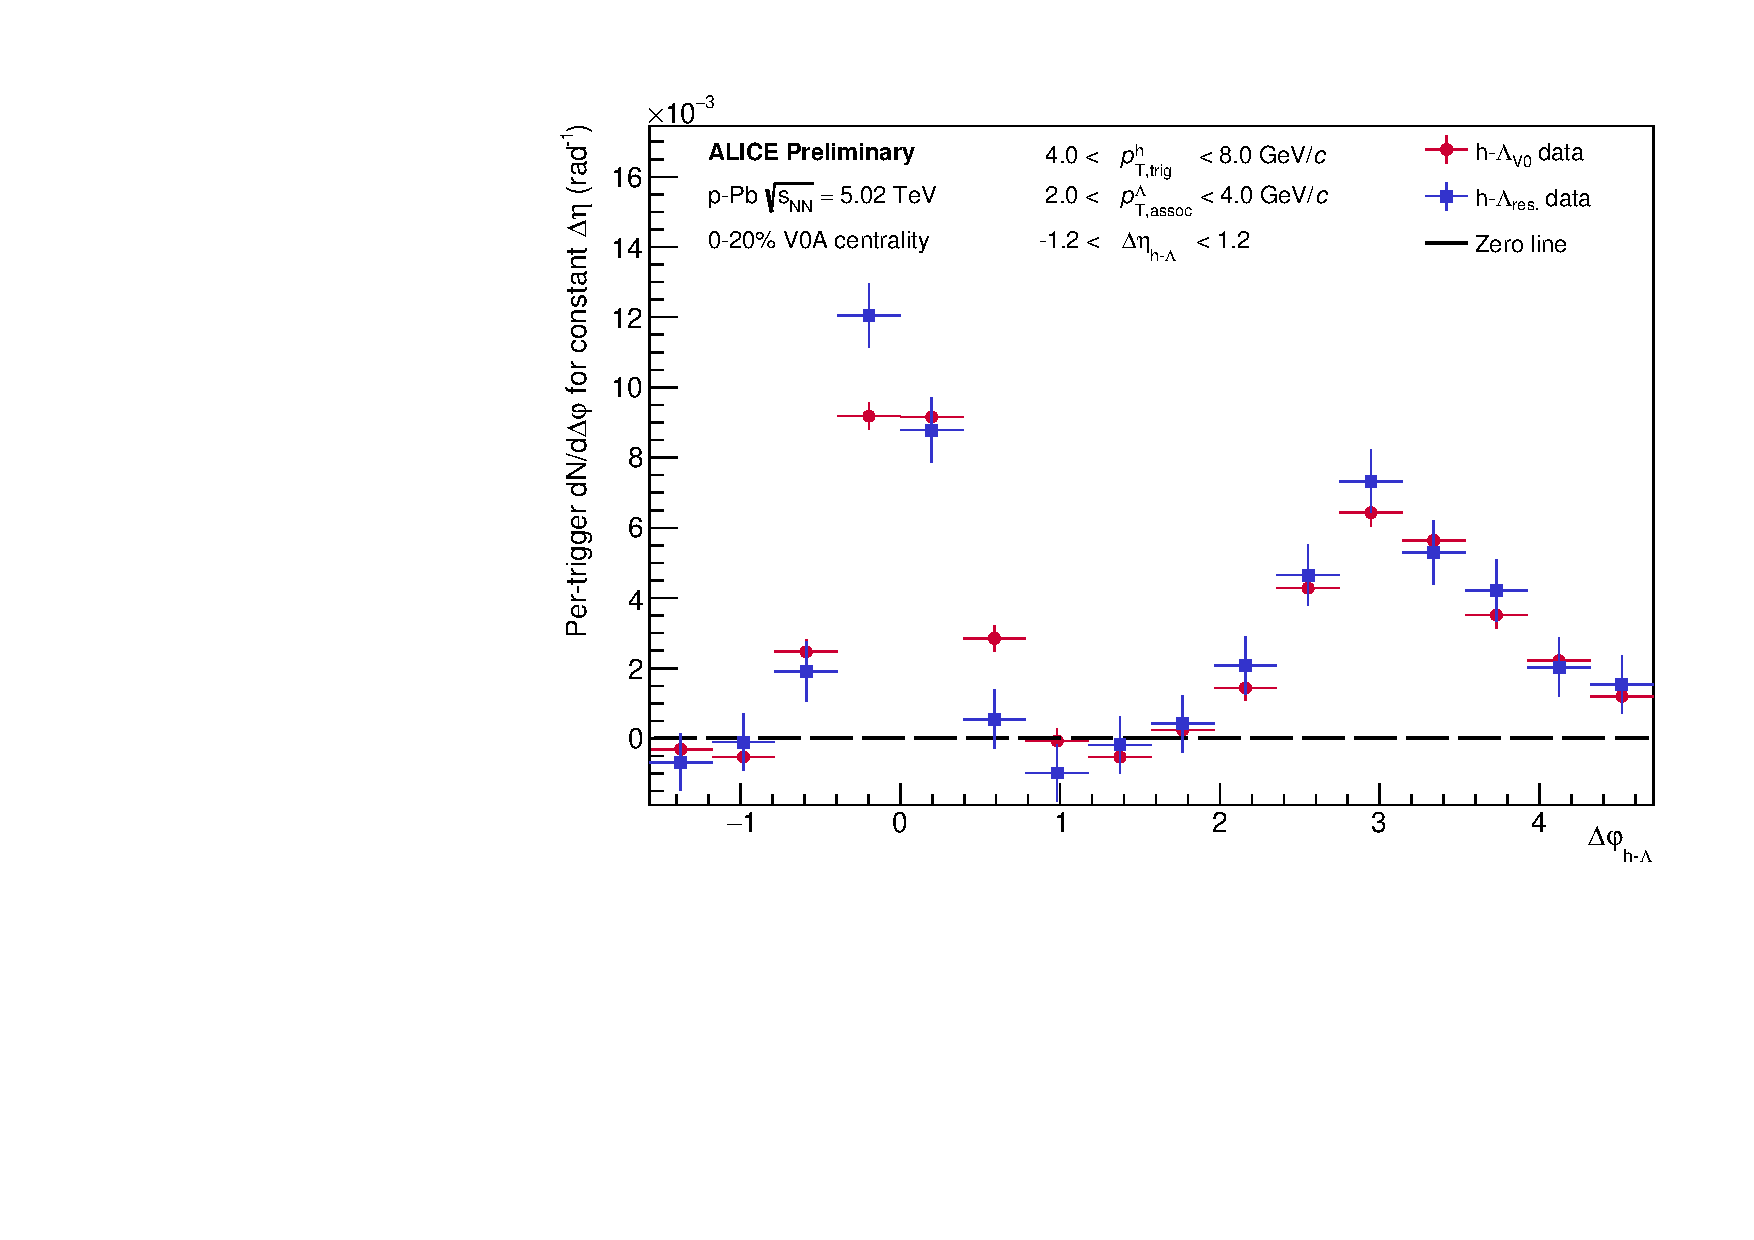
\includegraphics[width=0.32\textwidth]{figures/analysis/h_lambda_dphi_0_20_zeroed_rescomp.pdf}
    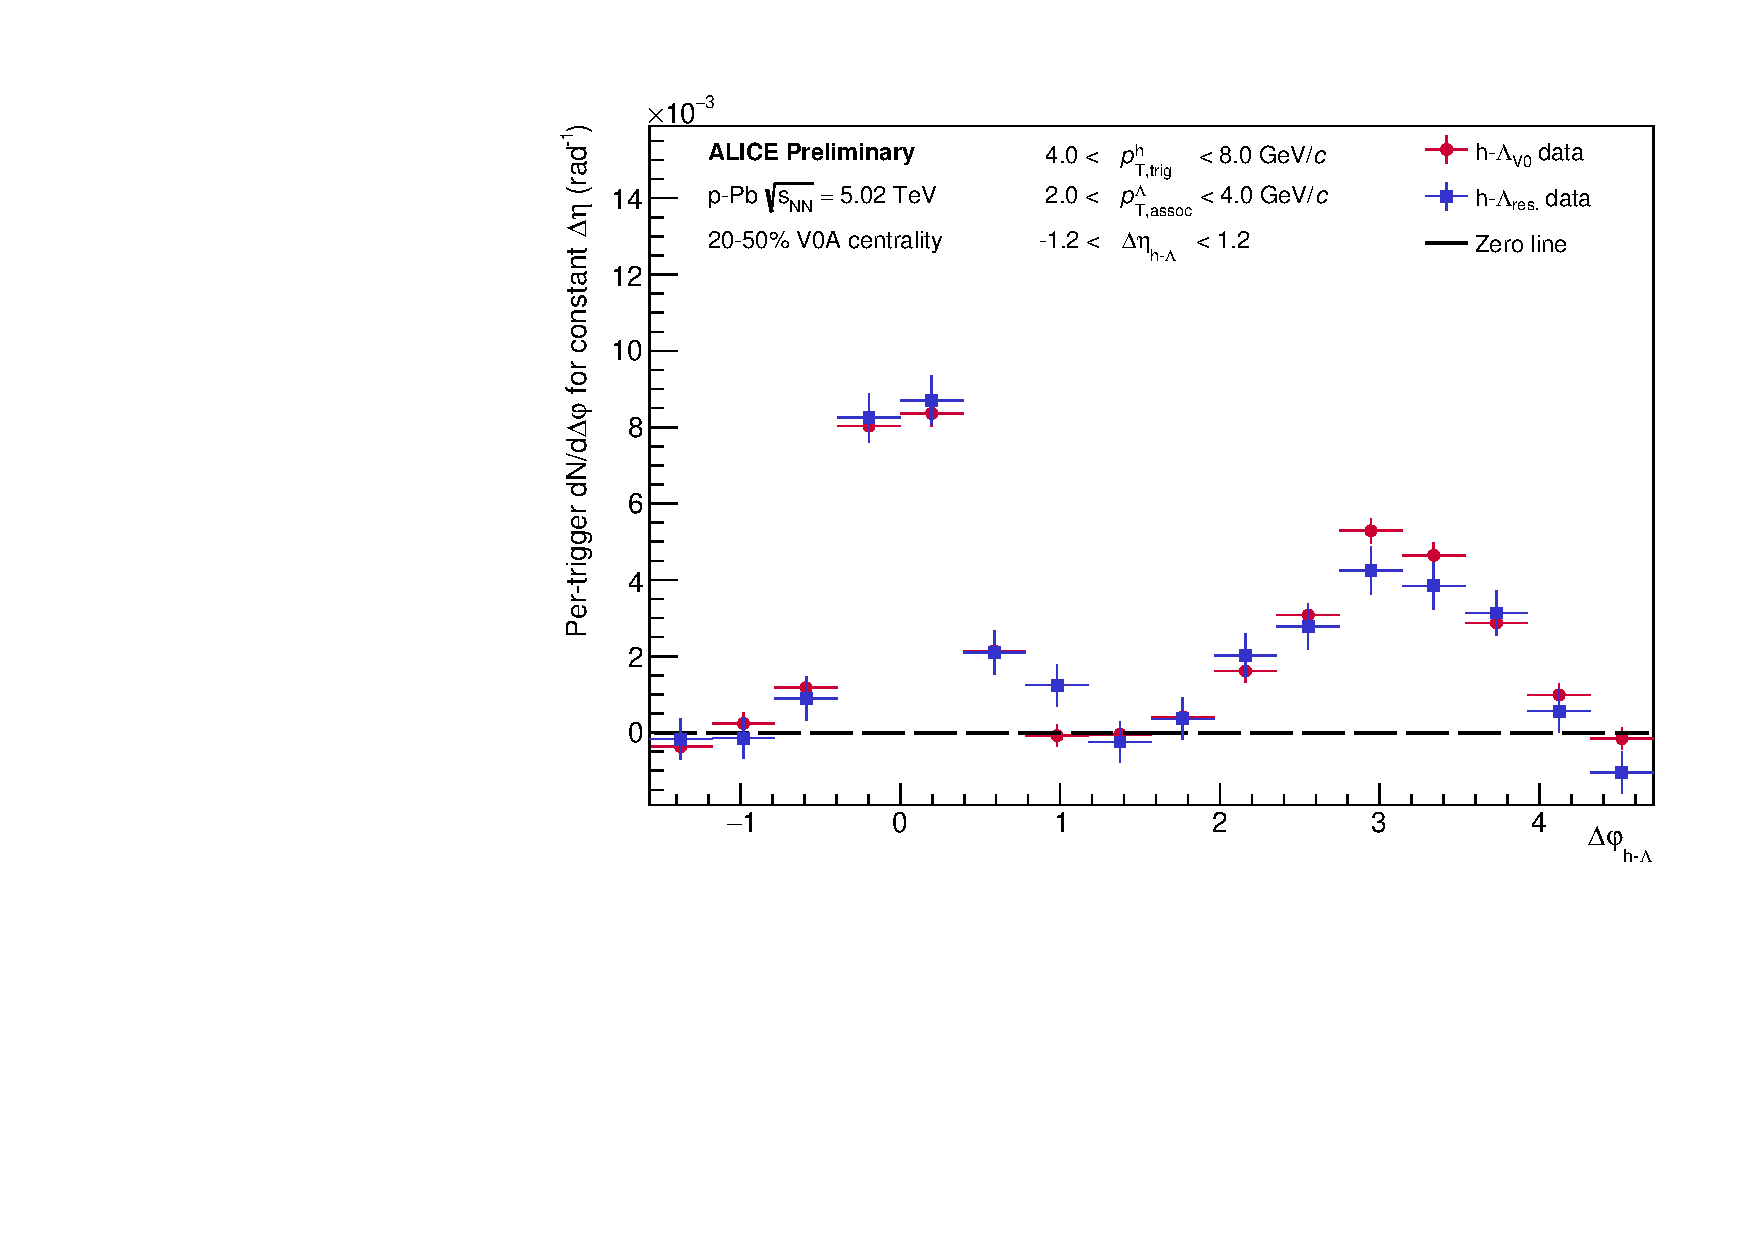
\includegraphics[width=0.32\textwidth]{figures/analysis/h_lambda_dphi_20_50_zeroed_rescomp.pdf}
    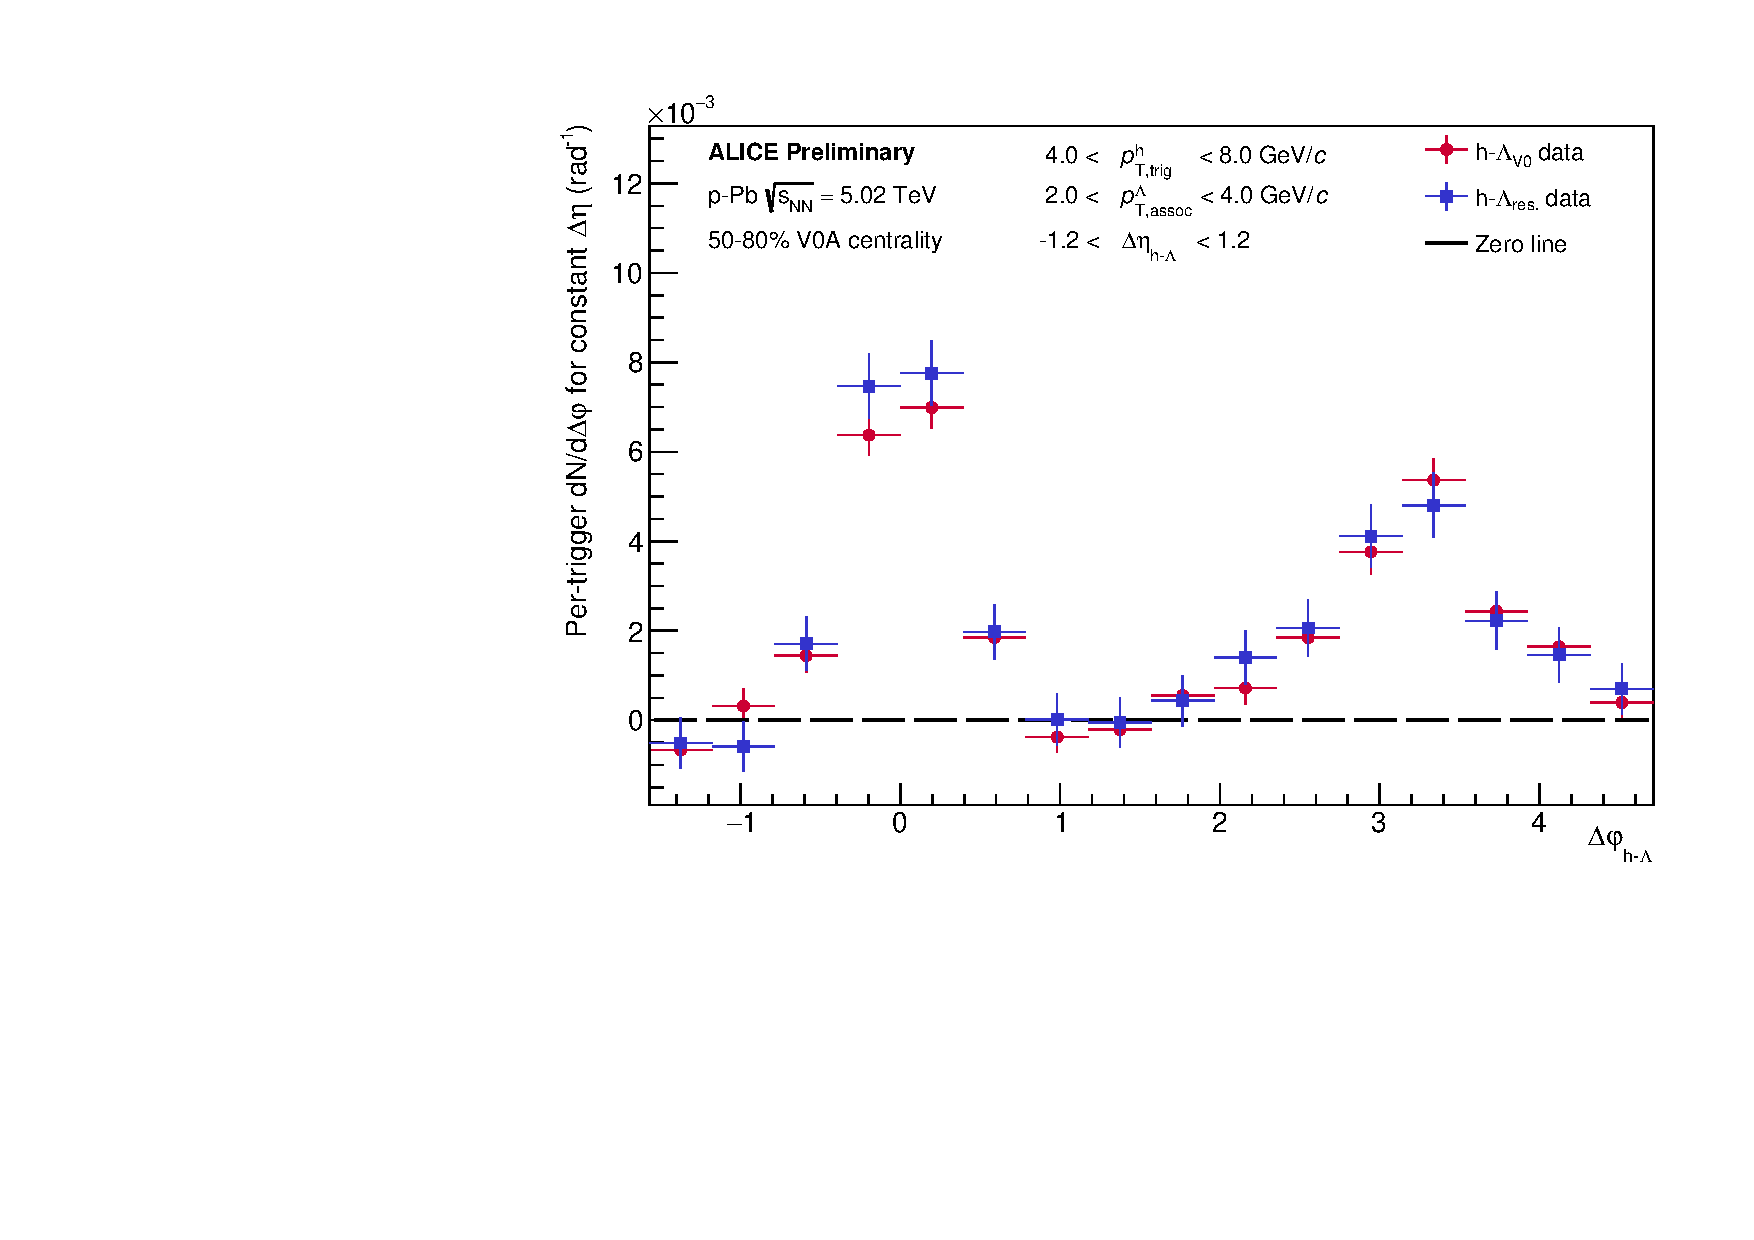
\includegraphics[width=0.32\textwidth]{figures/analysis/h_lambda_dphi_50_80_zeroed_rescomp.pdf}
    \caption{The final per-trigger h-$\Lambda$ $\Delta\varphi$ correlations for $\Lambda$s reconstructed using the resonance technique (blue) and the V$^{0}$-based technique (red) in the 0-20\% (left), 20-50\% (middle) and 50-80\% (right) multiplicity bins, taken in the associated momentum range $2.0 <$ \pt $< 4.0$ \GeVc, after the subtraction of the UE. The distributions show good agreement across all multiplicity bins, indicating that the V$^{0}$-based reconstruction technique is not introducing a bias in the correlation shape.}
    \label{fig:resonance_v0_dphi_comp_2}
\end{figure}

Additionally, the per-trigger near- and away-side pairwise yields and the (h-$\Lambda$)/(h-h) ratios with $\Lambda$s reconstructed using the resonance technique are shown in Figure~\ref{fig:resonance_final_results}. The results are qualitatively very similar to the nominal results, indicating that the resonance technique is a reasonably viable alternative to the \vz technique. However, due to the larger combinatorial background (and likely very large systematic uncertainties), the \vz technique is still the preferred method for \lmb reconstruction. 


\begin{figure}[ht]
\centering
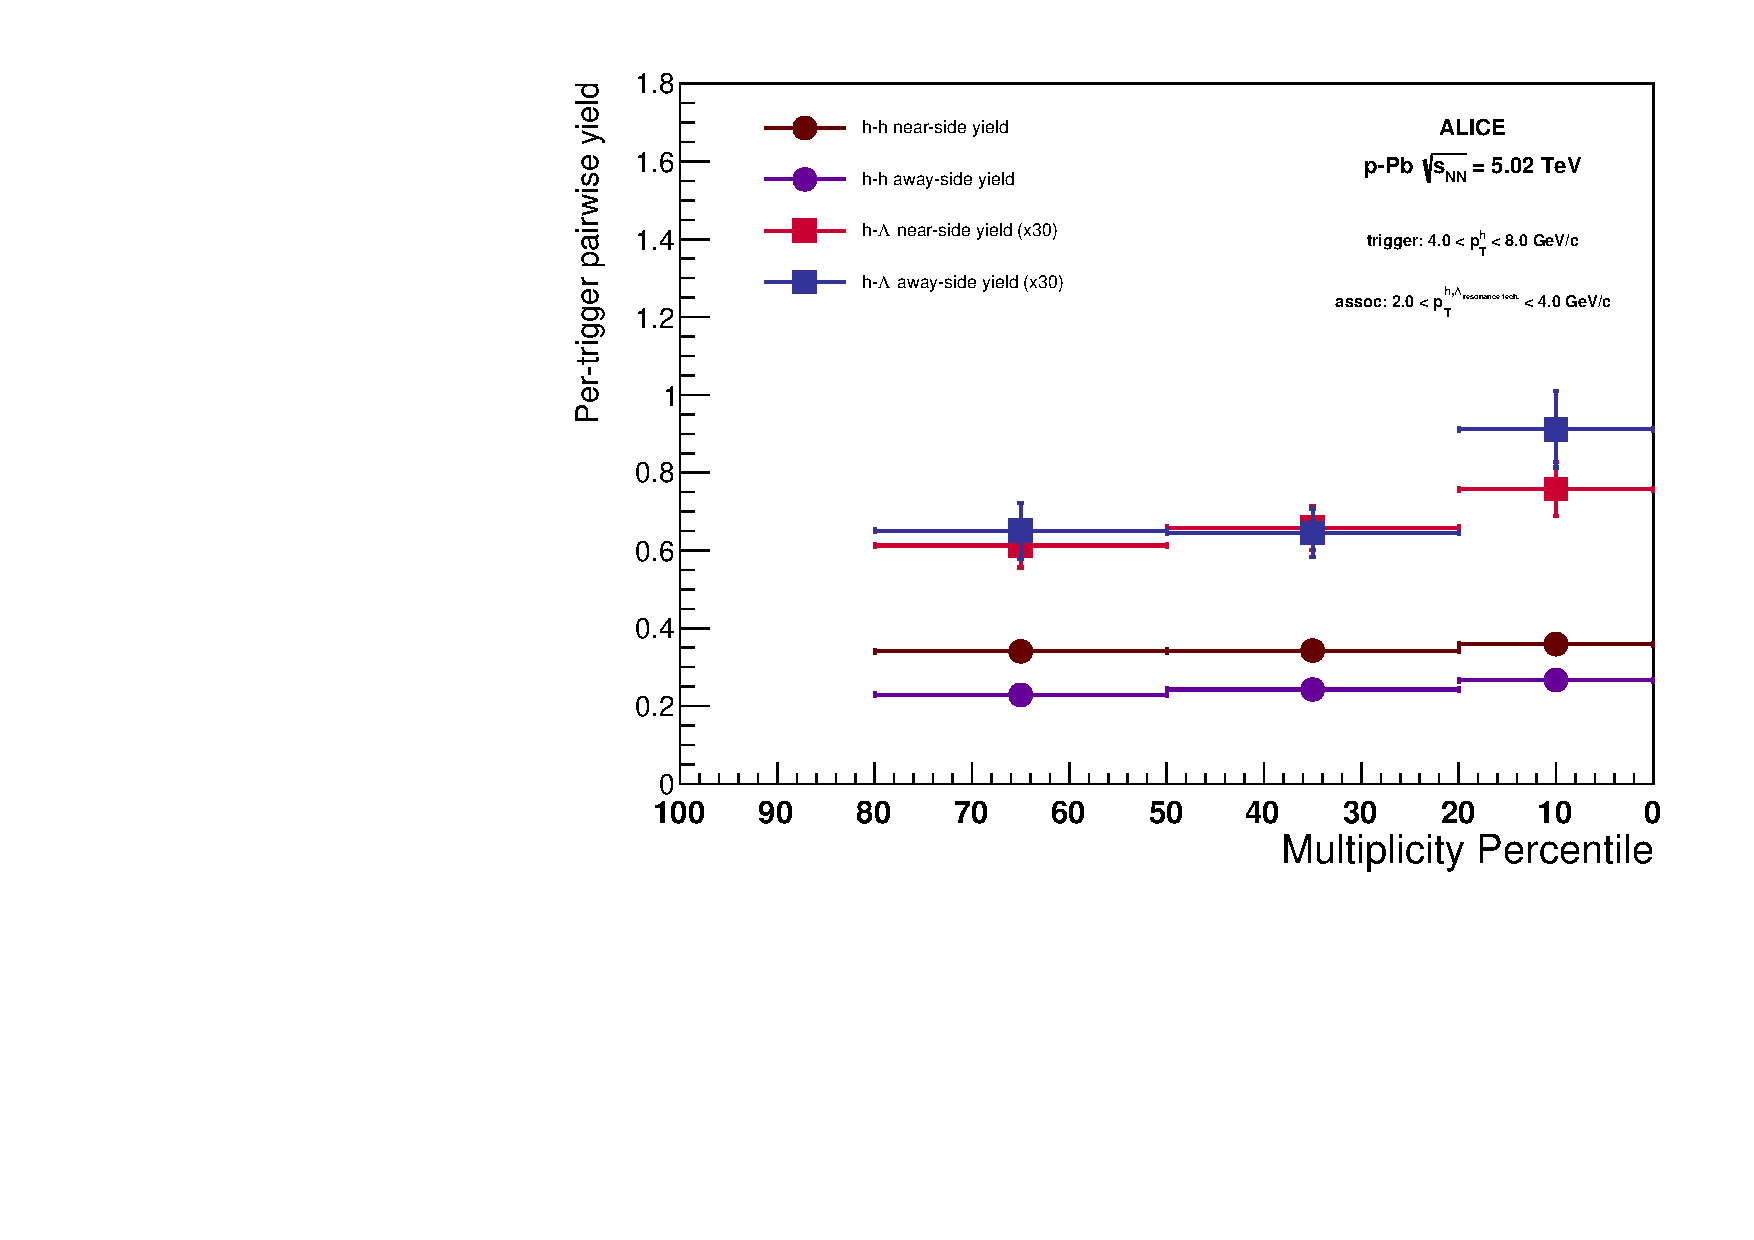
\includegraphics[width=0.7\textwidth]{figures/analysis/pairwise_plot_resonance.pdf}
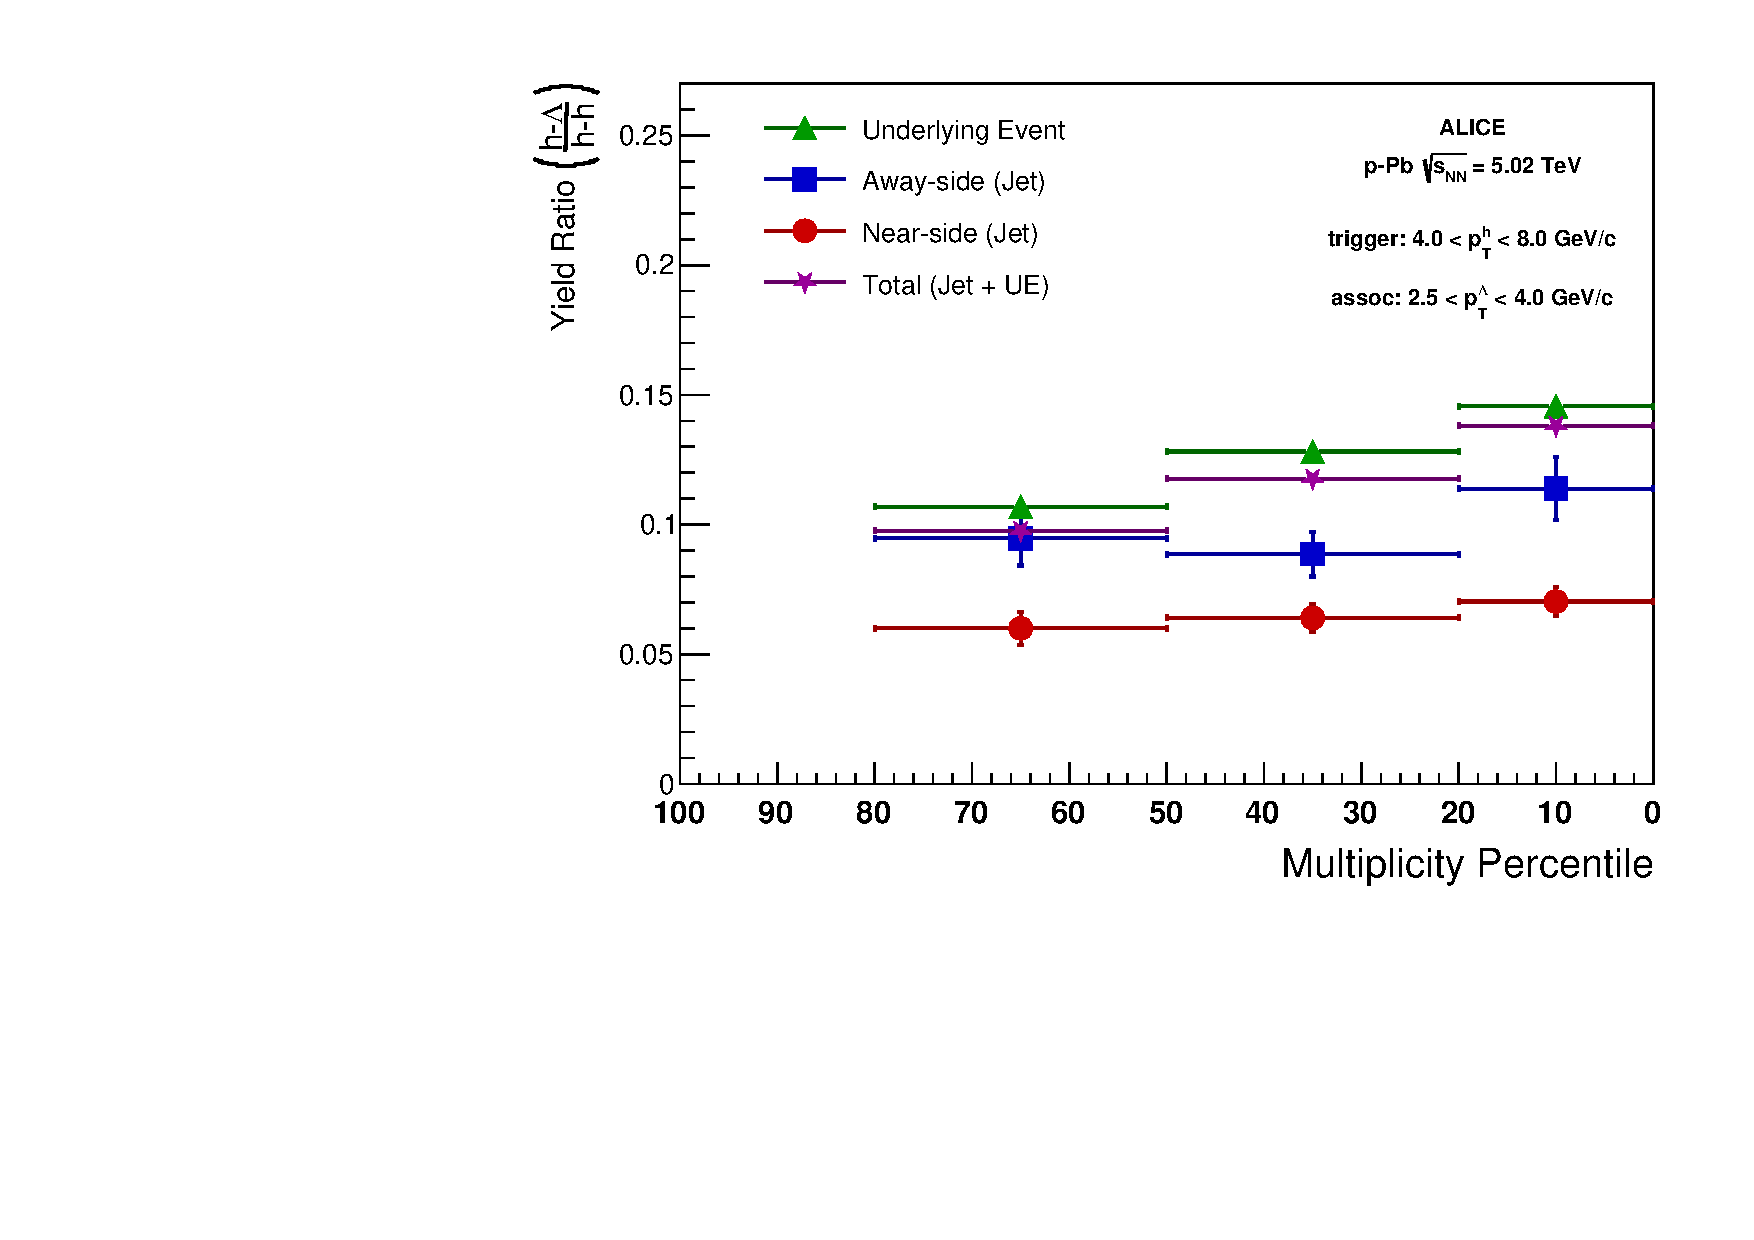
\includegraphics[width=0.7\textwidth]{figures/analysis/ratio_plot_resonance.pdf}
\caption{The final h-$\Lambda$ and h-h per-trigger pairwise jet yields (top) and (h-\lmb)/(h-h) yield ratios (bottom) vs. multiplicity in the associated momentum range $2.0 <$ \pt $< 4.0$ \GeVc for $\Lambda$s reconstructed using the resonance technique. The general trends are similar to the nominal \vz technique-based procedure, with larger statistical uncertainties.}
\label{fig:resonance_final_results}
\end{figure}